\chapter{LUX Post-Run 04 Calibration Campaign}
After the LUX Run4 WIMP-search was completed in June of 2016, the response of the detector was exercised using ER and NR calibration sources. The usual ER calibrations of krypton-83m\cite{lux_kr1,lux_kr2} and tritiated methane (CH$_3$T)\cite{lux_tritium} were performed, along with NR calibrations using the deuterium-deuterium (DD) neutron generator\cite{lux_dd1,lux_dd2}. In addition to these standard calibrations, there were additional techniques and sources used which were novel to the LUX detector. 


\begin{table}
\centering
    \begin{tabular}{ c | c | c | c | c }
    \hline
    Source & Date & $\tau_{1/2}$  & Energy & Rate \\ 
     &  & (days) & (keV) & (Hz) \\
    \hline \hline
    DD & -8/7, 8/22-8/23  & - & ($<$355) & - \\ 
    \hline
    Kr-83m & 8/2, 8/8, 8/10,  & 0.076 & 41.5  & 130\\ 
     & 8/17, 8/25, 8/31 & & &\\
    \hline
    Xe-131m & 8/9 & 12 & 163.9 & 10 \\ 
    \hline
    CH$_3$T & 8/18 & 0.3 & 0-18.1 & 50 \\ 
    \hline
    $^{14}$CH$_4$ & 8/23 & 0.3 & 0-156 & 100 \\ 
    \hline
    Rn-220 & 8/27, 8/29 & 0.3 & & 50 \\ 
    \hline
    Ar-37 & 8/31 & 0.3 & 35 & 70 \\ 
    \hline
    \hline
    \end{tabular}
    \caption{Table of sources which were used during the post-Run04 calibration campaign.}
\end{table}

The first novel calibration performed was a modification to the DD NR calibration. The rest of these new calibrations were to the ER response and will be the primary focus of this chapter, but we will pause here briefly to discuss the DD calibrations. The NR response of the LUX detector was measured using a beam of neutrons which was directed into the cryostat. These neutrons were generated using a commercially available DD generator, and were collimated using a gas filled conduit which was suspended in the water tank. Because the neutrons entering the detector have a known energy and direction, it is then possible to calculate the precise recoil energy of a neutron from the beam scattering off of a xenon nucleus, assuming the scattering angle is known. The calculation is the same for neutron-nucleus scattering as for WIMP-nucleus scattering:
\begin{equation}
E_R=\frac{E_nr}{2}[1-\cos(\theta)],
\end{equation}
where $\theta$ is the scattering angle in the center of mass frame, and $r=4M_AM_n/(M_A+M_n)^2$. The scattering angle in the lab frame can be easily measured for events where the scattered neutron interacts with a second xenon atom before exiting the detector, and for large nuclei such as xenon, the approximation $\theta_{CM}\approx \theta_{LF}$ can be made. The result of this procedure is a continuous NR recoil spectrum where the energy of each event is precisely known. These events will be located along the beam line, so will all be at roughly the same drift time. By moving the conduit up and down, the detector NR response as a function of drift time can be mapped out\cite{lux_dd1,lux_dd2}.
\begin{figure}[h!]
\centering
\begin{subfigure}{0.5\textwidth}
  \centering
  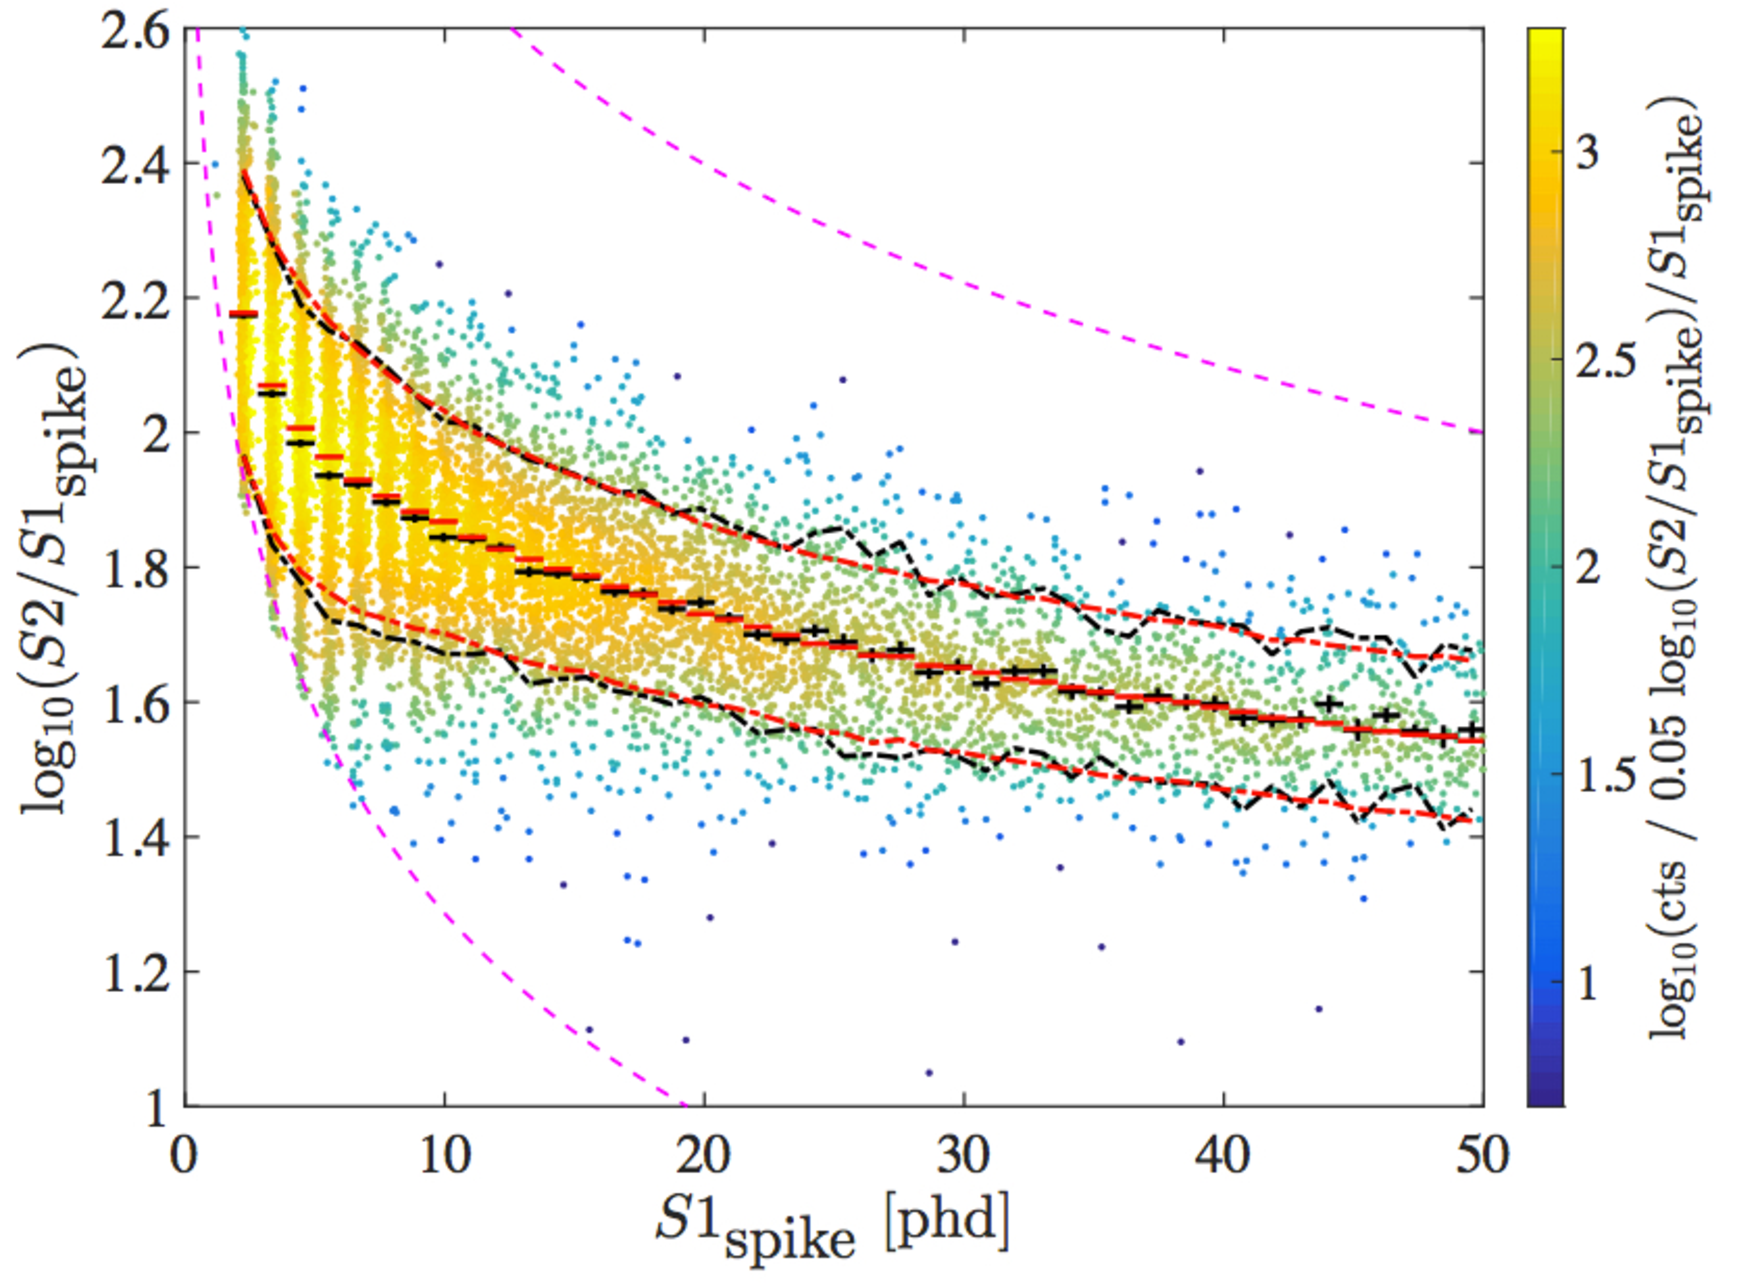
\includegraphics[width=\textwidth]{Figures/DDband.pdf}
  %\label{}
\end{subfigure}%
\begin{subfigure}{0.5\textwidth}
  \centering
  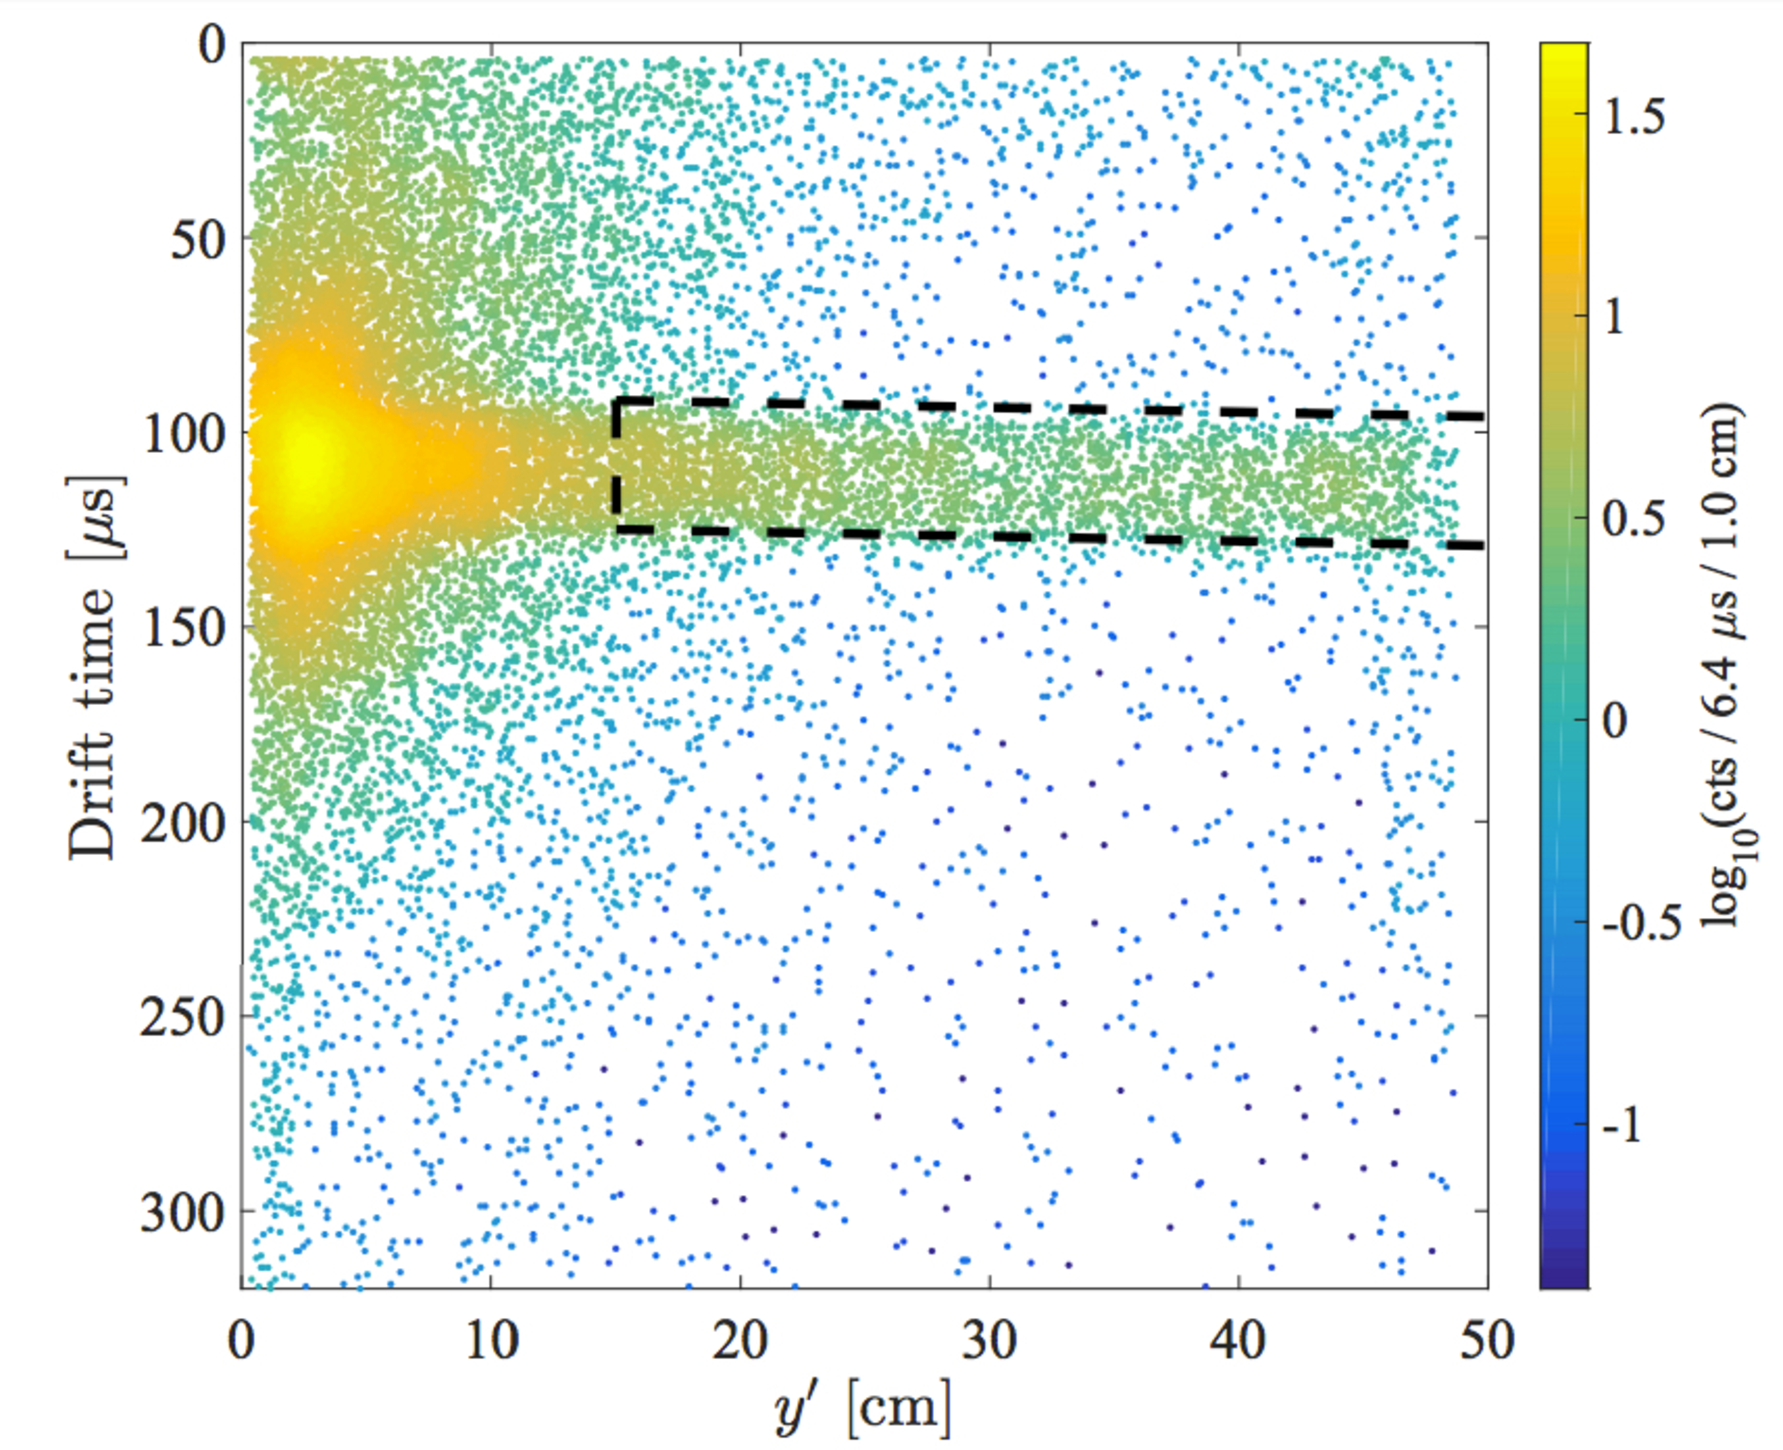
\includegraphics[width=\textwidth]{Figures/DDbeam.pdf}
  %\label{fig:intlin}
\end{subfigure}
\caption{Plots of the measured neutron beam line (left) and the NR recoil band (right) from a previous LUX D-D calibration. The $y'$ coordinate in the beam line plot is a transformation of the standard LUX $x$ and $y$ coordinates, such that it measures the horizontal distance along the beam line. The NR recoil band plot shows the continuous nature of the recoil spectrum. Figures taken from \cite{lux_dd2} }
\label{fig:ddplot}
\end{figure}

The novel modification to the DD calibration in the post-run 04 campaign was to first scatter the neutrons off of a D$_2$O target before sending them into the conduit. The only neutrons of a single, known, scattering angle will pass through the conduit, so this procedure effectively converts the 2.45 MeV mono-energetic neutron source to a 272 keV mono-energetic neutron source. The main portion of the post-Run4 DD campaign ended on August 7$^{th}$, although there was a final brief period of testing between August 22$^{nd}$ and 23$^{rd}$\cite{lux_dd1}.


On August 9$^{th}$, $^{131m}$Xe became the first of the non-standard, post-Run4 ER sources to be injected. Xenon-131m is a gamma-emitter with an energy of 163.93 keV and a half life of 11.84 days.\cite{nuclide}. The xenon-131m was collected from an iodine-131 pill in an otherwise empty stainless steel bottle and was injected using the tritium injection described in \cite{lux_tritium}. The 12 day half life of this source meant that all subsequent sources in the month long campaign have the $^{131m}$Xe line as a background. The $^{131m}$Xe line is sufficiently separated in energy from most of the other sources, so that this background will not have a significant effect. However, the $^{131m}$Xe line is only 8 keV above the $^{14}$C Q value of 156 keV and so obscures the highest-energy portion of the $^{14}C$ beta spectrum. This has two major effects on our analysis of the carbon-14 data. First, it limits us from probing the energy deposition properties of liquid xenon near the endpoint of the spectrum, and second, it provides an extremely useful reference point which can be used in energy calibration, efficiency corrections, and characterization of detector pathologies.

The tritium calibration was started on the 18$^{th}$, and the second new ER source, $^{14}$C was injected five days later on the 23$^{rd}$. Both of these sources rely on the injection of radio-labelled methane and are purified out by the LUX getter with a time constant of about 10 hours. This means that the tritium will have been reduced by about 12 e-folds, or a factor of 150,000, by the time the $^{14}$C was injected. Since the amount of tritium events in this injection was about 1 million, there should be an overlap of $<$10 events in the $^{14}$C injection.

The next source injected was radon-220. There were two injections, each with peak activity of about 50 Hz on the 27$^{th}$ and 29$^{th}$. Radon-220 is part of the thoron-232 decay chain, which ends with the stable lead-208. The transition time from $^{220}$Rn to $^{208}$Pb is dominated by the $\beta^-$ decay of $^{212}$Pb to $^{212}$Bi, which has a half life of about 10.6 hours. 

A 70 Hz injection of $^{37}$Ar took place on the 31$^{st}$, about 3 days after the second radon-220 injection. This meant that there was about 1 Hz of $^{212}$Pb remaining in the detector. The most common and most energetic $^{37}$Ar decay will deposit 2.8 keV into the xenon via x-ray. The low energy of the decay means that the $^{37}$Ar events will be well separated from the MeV-level alphas and betas of $^{212}$Pb and its daughters. The high rate and 35 day half life of the injected $^{37}$Ar meant that this was the final injection performed in the post-Run4 campaign, and was in fact the last physics data collected by the LUX detectors.

The rest of this chapter will focus on the $^{131m}$Xe, $^{37}$Ar, and $^{14}$C sources. We will also present a review $^{83m}$Kr and $^{3}$H. This particular suite of sources is exciting in the fact that it includes two continuous beta spectra, which can be used to map out xenon ER yields from 140 keV down to threshold, as well as three ER lines that can be used to correct for position dependent detector efficiency and examine systematic pathologies.
\begin{figure}[h!]
\centering
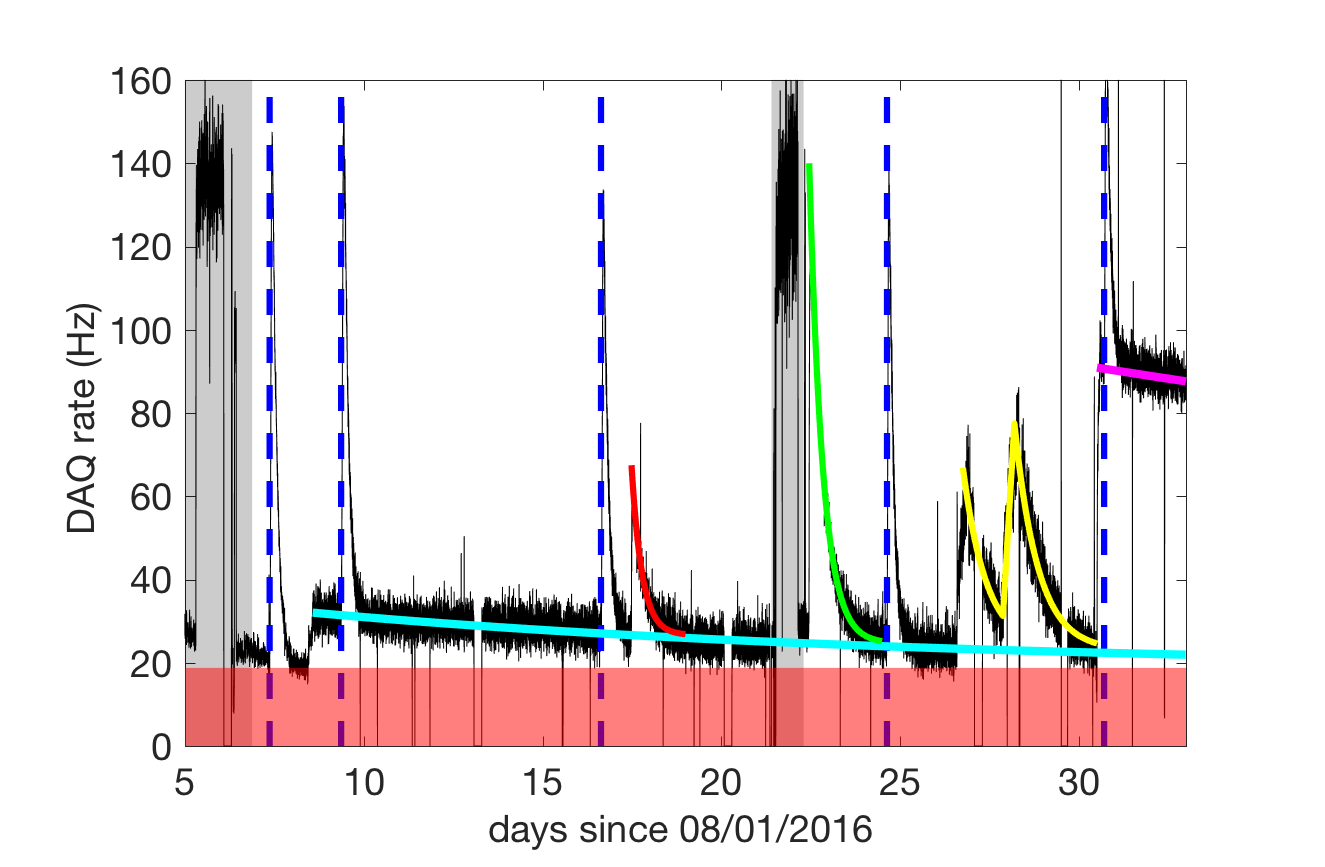
\includegraphics[width=\textwidth]{Figures/post_Run4_DAQrate.eps}
\caption{The black line shows the DAQ rate for the post-run04 injection campaign. The red shaded region shows the constant baseline, while the grey shaded regions show the DD NR-calibration campaign. The vertical dashed blue lines show the times of standard $^{83}$Kr$_m$ injections. The cyan, red, green, yellow, and magenta lines trace the $^{131m}$Xe, $^{3}$H, $^{14}$C, $^{220}$Rn, and $^{37}$Ar activities, respectively.} 
\label{fig:DAQrate}
\end{figure}


\section{Data Selection}
There were several preliminary data selection cuts applied to isolate the $^{37}$Ar K-capture, $^{131m}$Xe, $^{83m}$Kr, $^{3}$H, and $^{14}$C events. The time interval which these events were drawn from is  August 17$^{th}$ until September 3$^{rd}$. In figure \ref{fig:DAQrate} this corresponds to the third krypton injection at T=16.6 days, until the end of data taking. The periods of DD generator and $^{220}$Rn activity were excluded (from T=21.4 to 22.3 days and T= 26.8 to 30.5 days, respectively). There was also a period of time after the $^{14}$C calibration, from T=24.5 to 26.8 days, where one of the PMT's was misbehaving. This time period, which included the fourth krypton injection, was also rejected.


\subsection{Single-Scatter Cut}\label{sec:sscut}
The fully processed LUX data is organized into events. These events span a 500 microsecond window on either side of an initial trigger and is subdivided into ten ``pulses'' which are categorized as S1, S2, single-liquid-electron, single-photoelectron, or other. We would like to make a selection cut on single scatter events; events in which there is exactly one interaction within the detector which is located at a point position. The simplest cut one can make to this end is to keep only those events which contain exactly one S1, which is followed by exactly one S2. This cut, however, turns out to have an energy dependence, especially above 100 keV, which will alter the shape of our continuous spectra. 

We can quantify this energy dependence by looking at the Xe-131m peak. A cut on single-S1 events will only accept about about 77\% of Xe-131m events, while a cut on single-S2 will accept only about 68\%. Combining these cuts forms a naive single scatter cut, and accepts only about 61\% of the xenon-131m events. Conversely, the single scatter cut for carbon-14 events from threshold up to about 50 keV has greater than 90\% acceptance.
\begin{figure}[h!]
\centering
\begin{subfigure}{0.5\textwidth}
  \centering
  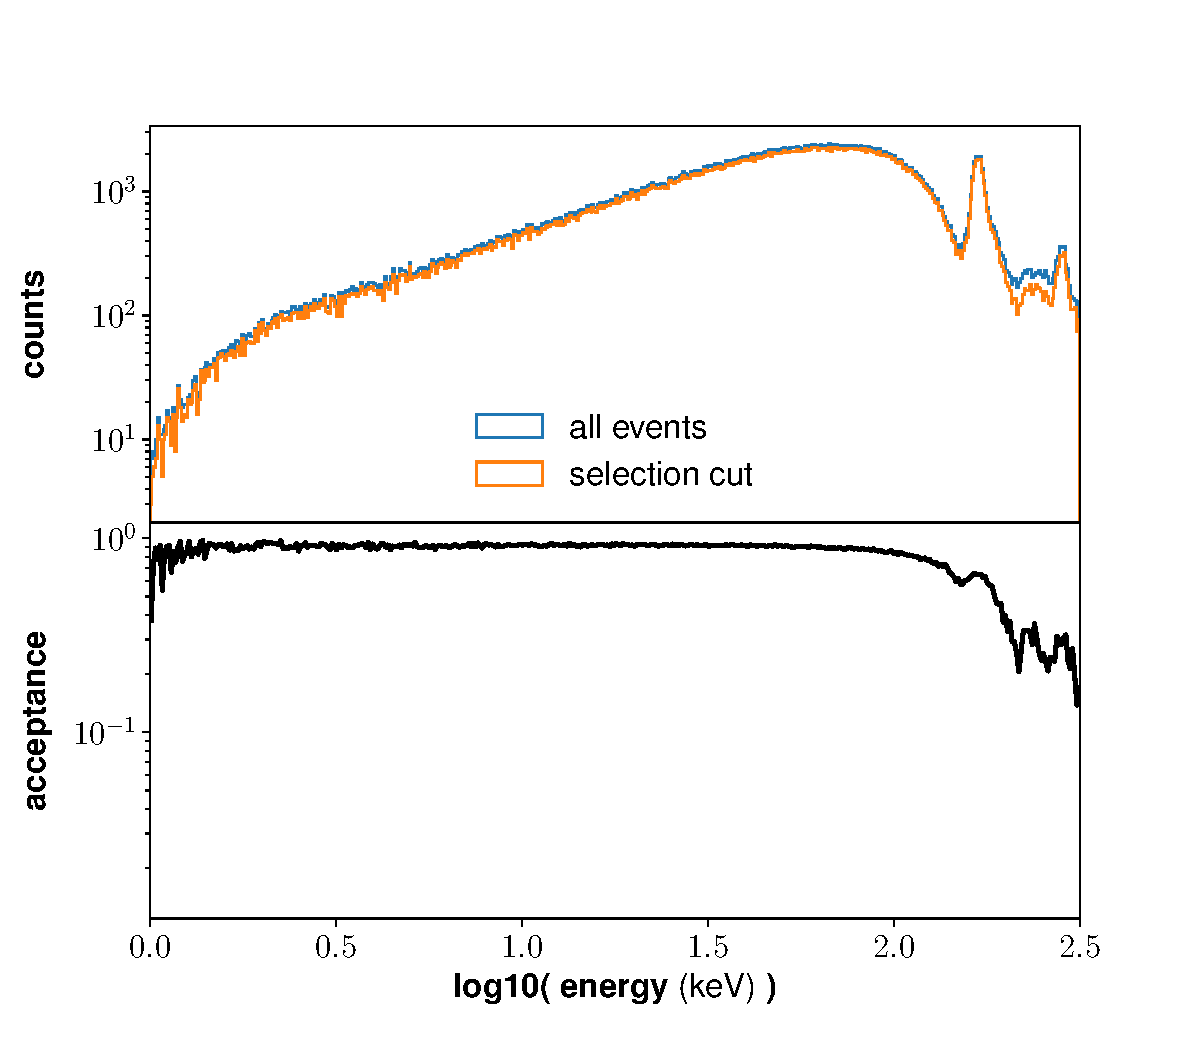
\includegraphics[width=\textwidth]{Figures/DataSelection_singlescatter}
  %\label{}
\end{subfigure}%
\begin{subfigure}{0.5\textwidth}
  \centering
  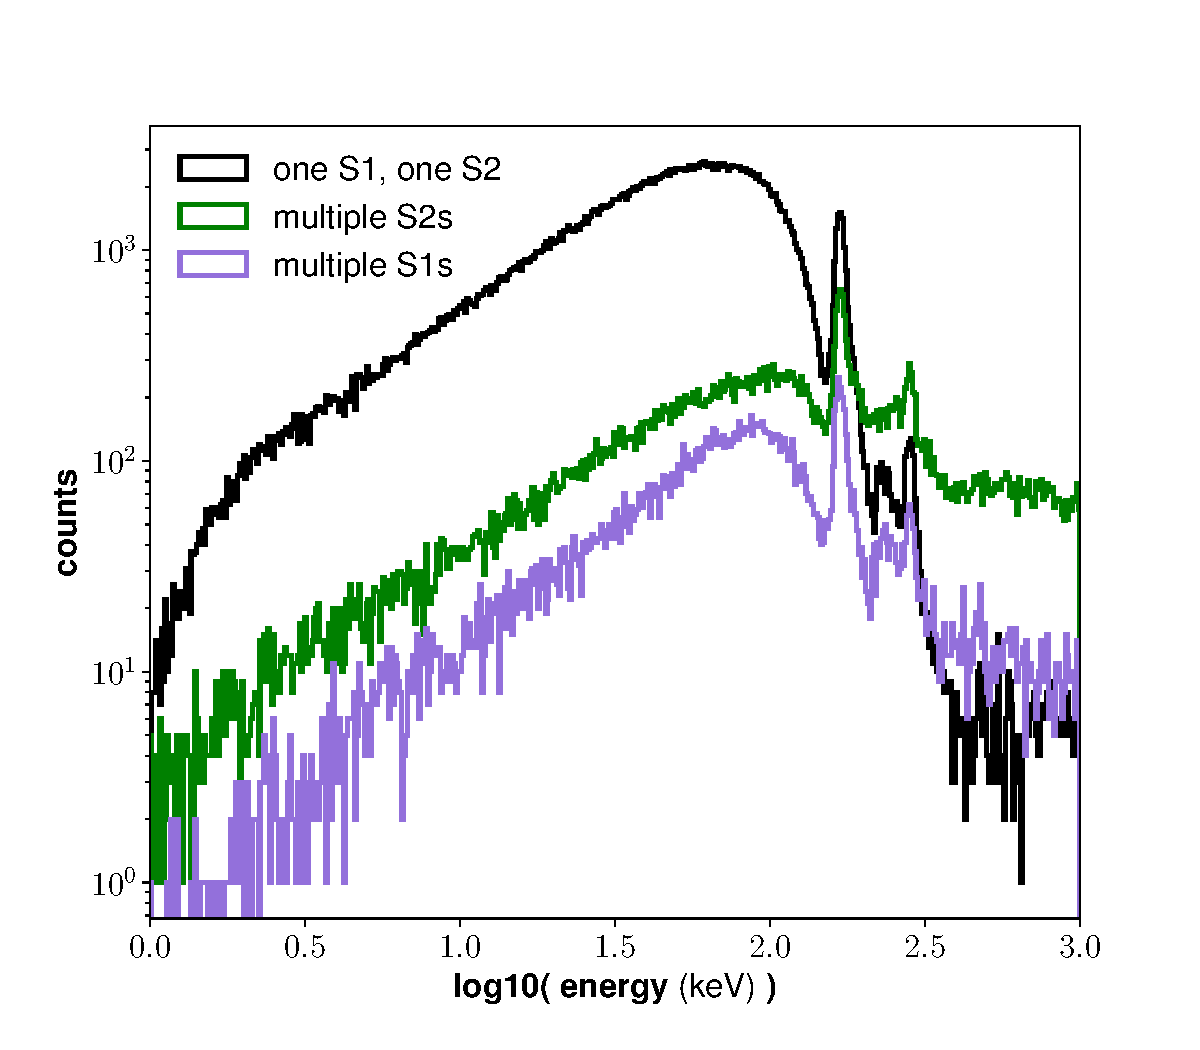
\includegraphics[width=\textwidth]{Figures/DataSelection_multiS1S2}
  %\label{fig:intlin}
\end{subfigure}
\caption{Visualization of the energy dependence of a single-scatter cut on carbon-14 and Xe-131m events. The loss of such a cut quickly rises above about 50 keV, to the point  where there is less than 10\% acceptance above about 500 keV.}
\label{fig:ssplot}
\end{figure}

The loss of acceptance at higher energy is largely dominated by the same pathology that is thought to cause S2 tails, which will be discussed in a later section. Electron trains are extended streams of electrons which are extracted from the liquid surface, persisting for millisecond time-scales. These trains seem to be seeded by S2s, and have a larger effect on higher-energy events. When an electron train is has a large enough rate, several of these electrons can pile up in a single pulse causing it to be classified as an S2. These secondary S2s will cause the event to fail the single scatter cut, and since the high-rate tails are more likely at higher energy, this will introduce an energy-dependence to the single-scatter cut.

For these reasons, we developed a more nuanced cut that allows for any number of S1s and S2s to be present. We first enforce the condition that there is at least one S1 before the first S2. We then cut on the ratio of the area of the first S2 to the sum of all of the S2 areas contained in the event. The idea is that we want the first S2 to contain greater than 93\% of the total S2 area, while allowing for subsequent smaller S2s to be present. We apply the cut to the S1s, however we only include S1s that occur before the first S2 in our total area sum.  
\begin{figure}[h!]
\centering
\begin{subfigure}{0.5\textwidth}
  \centering
  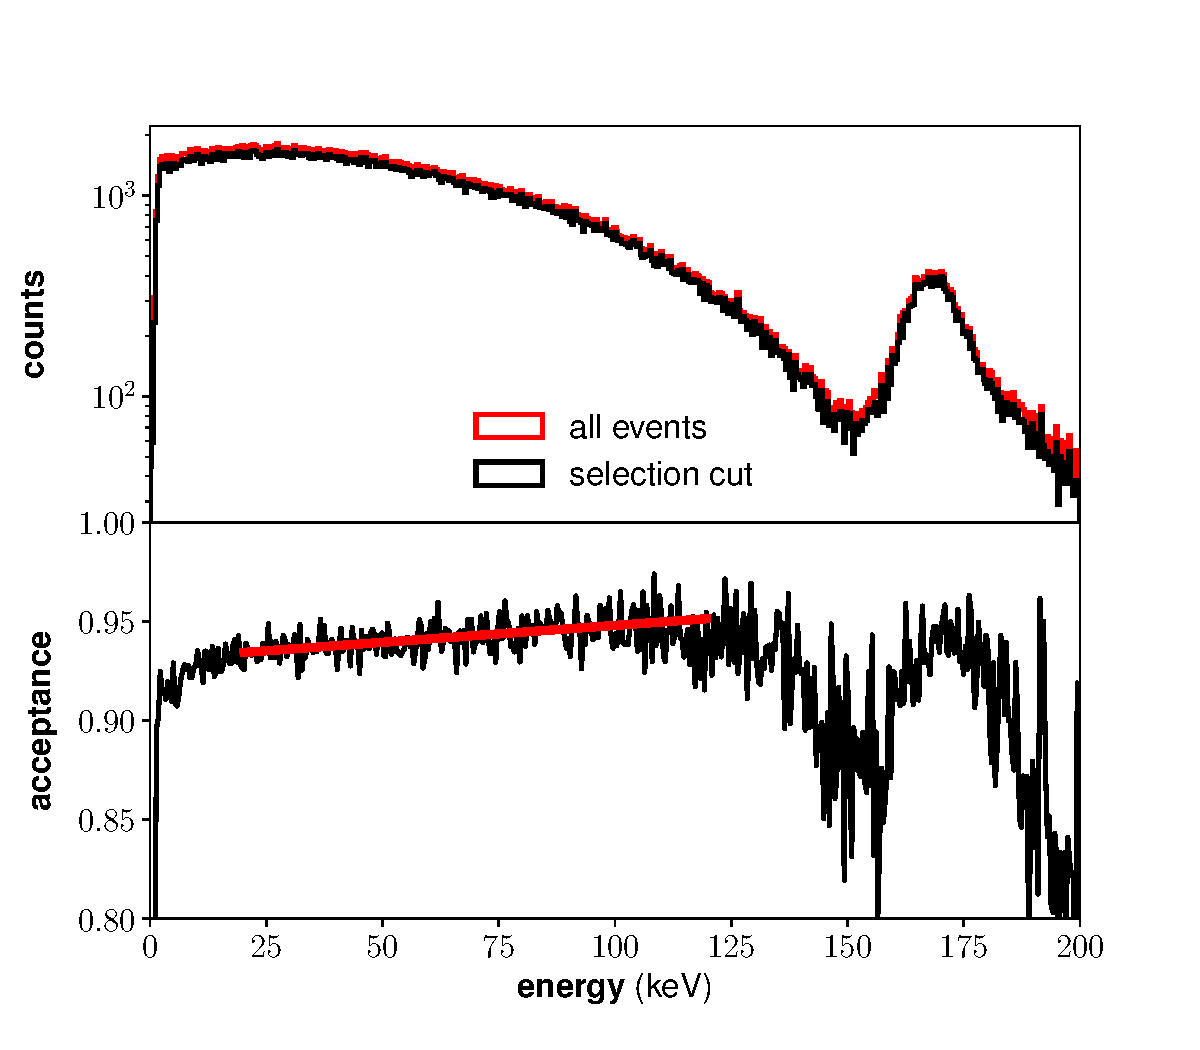
\includegraphics[width=\textwidth]{Figures/DataSelection_singlescatter_new}
  %\label{}
\end{subfigure}%
\begin{subfigure}{0.5\textwidth}
  \centering
  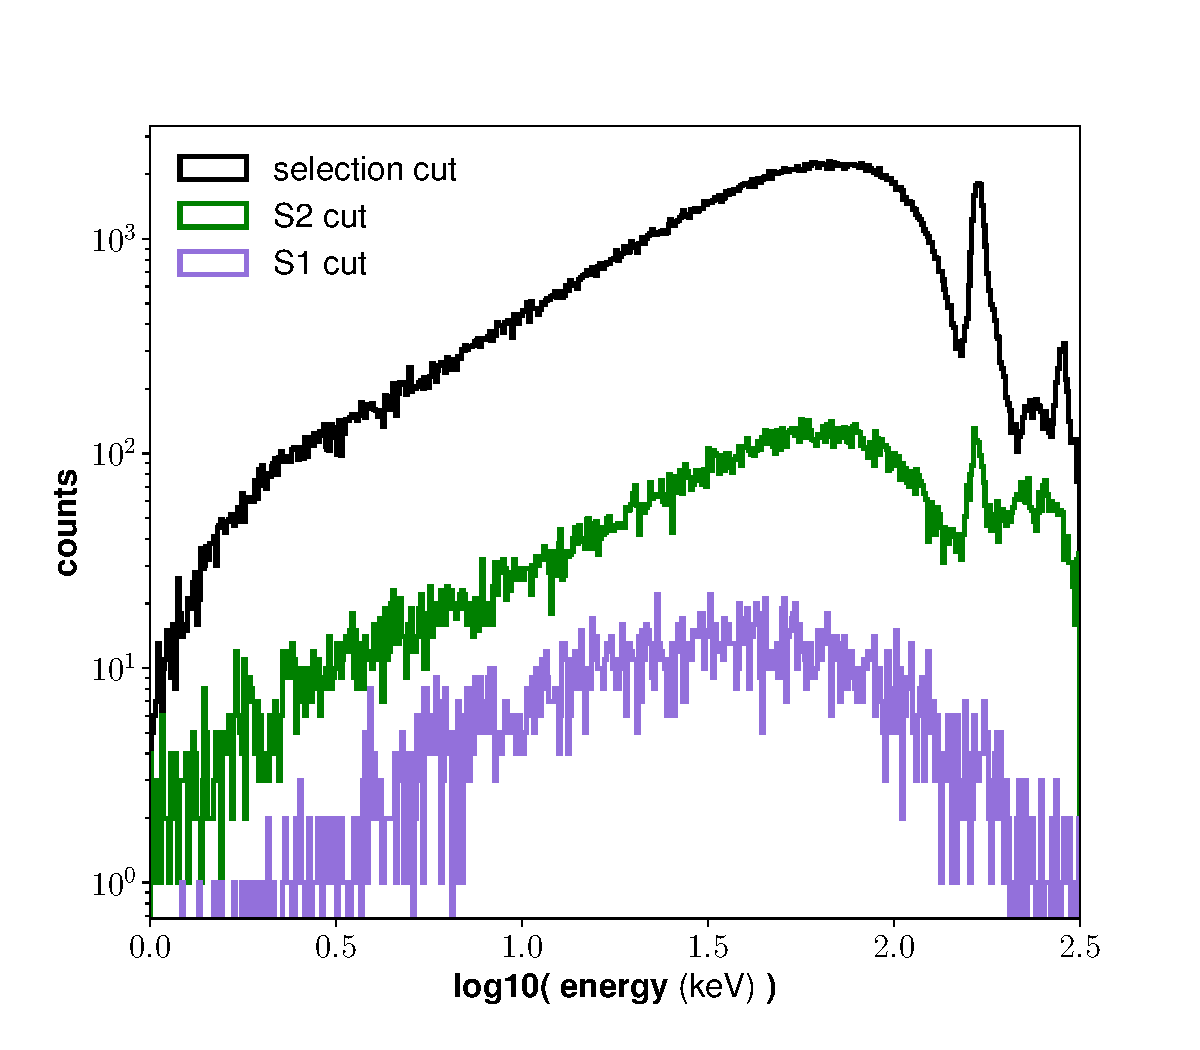
\includegraphics[width=\textwidth]{Figures/DataSelection_multiS1S2_new}
  %\label{fig:intlin}
\end{subfigure}
\caption{Visualization of the modified single scatter cut. This cut has a significantly better acceptance than the 1-S1, 1-S2 cut shown in figure \ref{fig:ssplot}. The acceptance of Xe131 events has been improved from 61\% to about  92\%. Similarly the acceptance for C-14 events is greater than 90\% across the entire energy range. There is a slight slope of 0.17 MeV$^{-1}$ to the acceptance of C-14 events which is indicated by the red best-fit line in the lower left panel. }
\label{fig:ssplot_new}
\end{figure} 

This cut has a significantly better acceptance than the 1-S1, 1-S2 cut. The acceptance of Xe131 events is improved from 61\% to about  92\%. Similarly the acceptance for C-14 events is greater than 90\% across the entire energy range. There is a slight slope of 0.17 MeV$^{-1}$ to the acceptance of C-14 events which is indicated by the red best-fit line in the lower left panel. This slope will introduce a systematic error in our measurement of the carbon-14 non-statistical shape factor, which will be described in section \ref{sec:shape_factor}. 

\subsection{Radial Selection Cut}
We would like to be able to eliminate events close to the wall from our analysis. The LUX Run4 and post-Run4 drift field was highly non-uniform in the z-coordinate, so there must be a drift time dependence added to any radial event-selection cut. There is, to a lesser degree, some non-uniformity in the radial and azimuthal directions as well. Since we would like to make a radially symmetric selection cut, we can to, first order, ignore the radial dependence. The radial cut was defined by first dividing the detector into 5$\mu$s drift time bins. Each drift time bin was re-centered around the mean S2-space x and y positions. These re-centered positions were then divided into 36 $\phi$ bins. We used the assumption that the argon-37 events will be distributed uniformly in radius-squared to define the cut position for each of these $\phi$ bins. We define $r_{cut}(dT,\phi)$ such that 77\% of events in the associated bin will have $r<r_{cut}(dT,\phi)$. The true radius of this event should be $\sqrt{0.77}R_{wall}=(0.877)\cdot (25 \text{\ cm})=21.9 \text{\ cm}$. The values of $r_{cut}(dT,\phi)$ should then all be about 3 cm from the wall. We apply this cut in each drift time bin ($dT_i$) by performing a linear interpolation between the values of $r_{cut}(dT_i,\phi)$ and cutting out events with radii greater than the interpolated values.
\begin{figure}[h!]
\centering
  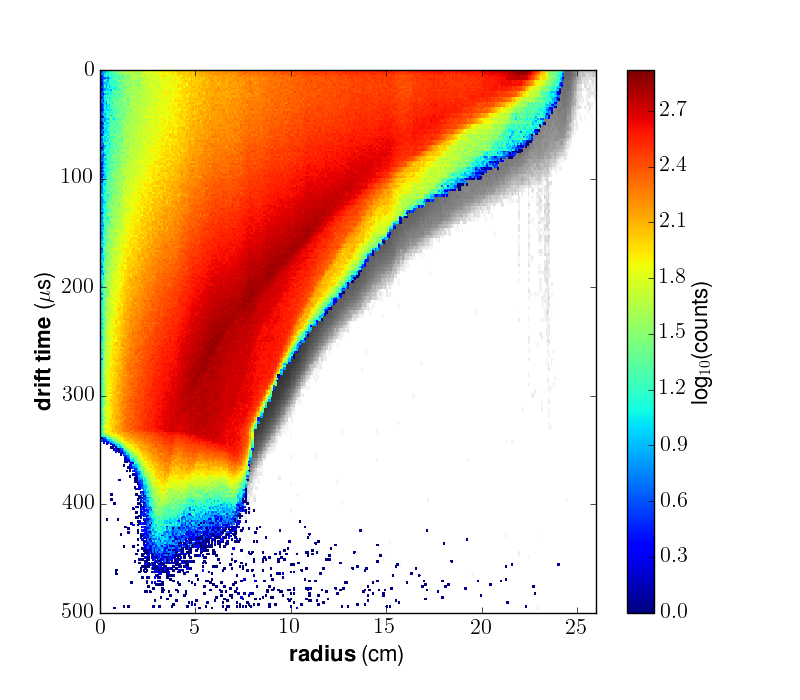
\includegraphics[width=\textwidth]{Figures/xycut_dt.png}
\caption{Visualization of the radial cut derived from the $^{37}$Ar data. The greyscale maps show the data without any position cuts, while the overlaid heat-maps show the selected by the radial cuts. }
\label{fig:xycut_dt}
\end{figure}
\begin{figure}[h!]
\centering
  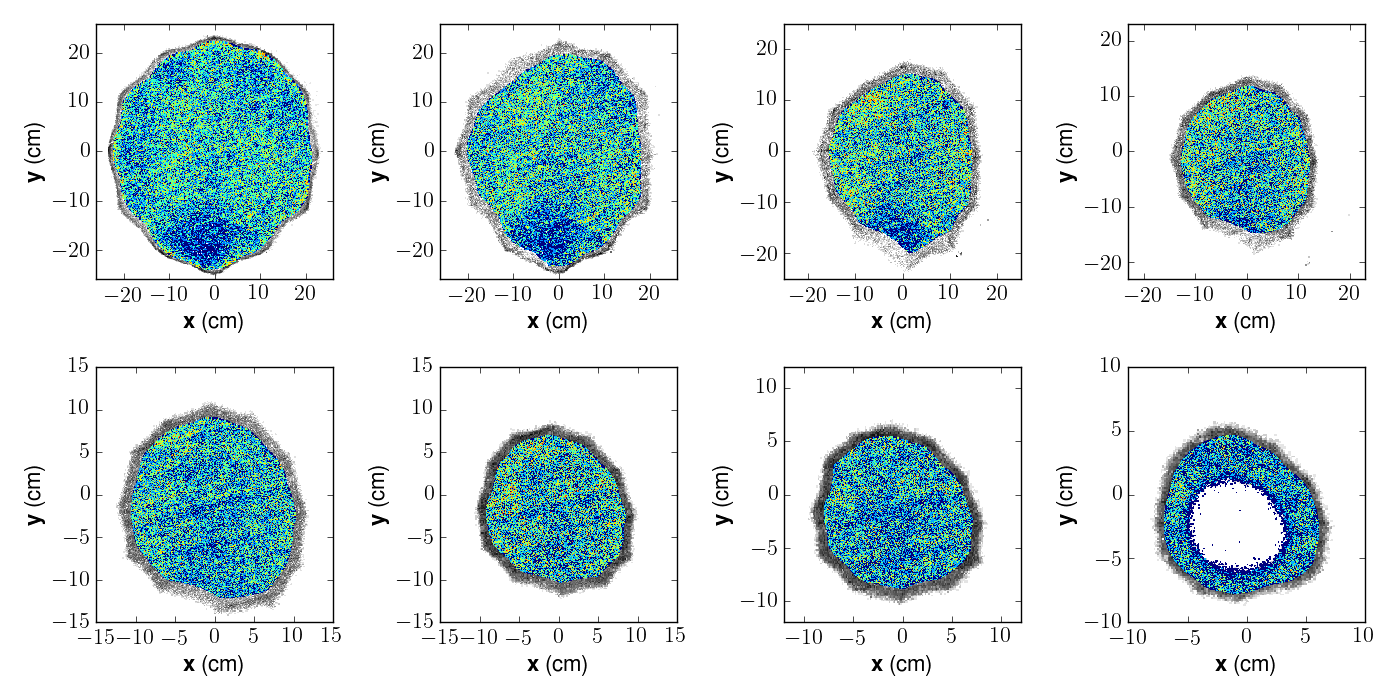
\includegraphics[width=\textwidth]{Figures/xycut_xy.png}
\caption{Selected 5 $\mu$s drift time slices used in the $^{37}$Ar drift time section cut. The greyscale maps show the data without any position cuts, while the heat-map shows the selected by the radial cuts. From top left to bottom right, the drift time of the cots are 20 $\mu$s, 50 $\mu$s, 100 $\mu$s, 150 $\mu$s, 200 $\mu$s, 250 $\mu$s, 300 $\mu$s, and 350 $\mu$s. The linear diagonal lines that can be seen in the heat-maps are physical features created by the grids.}
\label{fig:xycut_xy}
\end{figure}

\subsection{Electric Field Selection Cut}\label{sec:fieldbins}
In the next chapter, we will be interest in making measurements as a function of field. To that end, we have divided the detector into 13 electric field bins. To construct these bins, we first assign an electric field value to each event by using the SciPy ``LinearNDInterpolator'' tool\cite{scipy} on the the field-map described in section \ref{sec:efield}. We select electric-field bins such that the assigned field of each event, $\mathcal{E}$, is within 10\% of the center of some field bin, $\mathcal{E}_{ctr}$. The electric field cut applied to the  $i^{th}$ bin would then be:
\begin{equation}\label{eq:ebin_e}
0.9\cdot \mathcal{E}_{ctr,i}< \mathcal{E} < 1.1\cdot \mathcal{E}_{ctr,i}.
\end{equation}
\begin{figure}[h!]
\centering
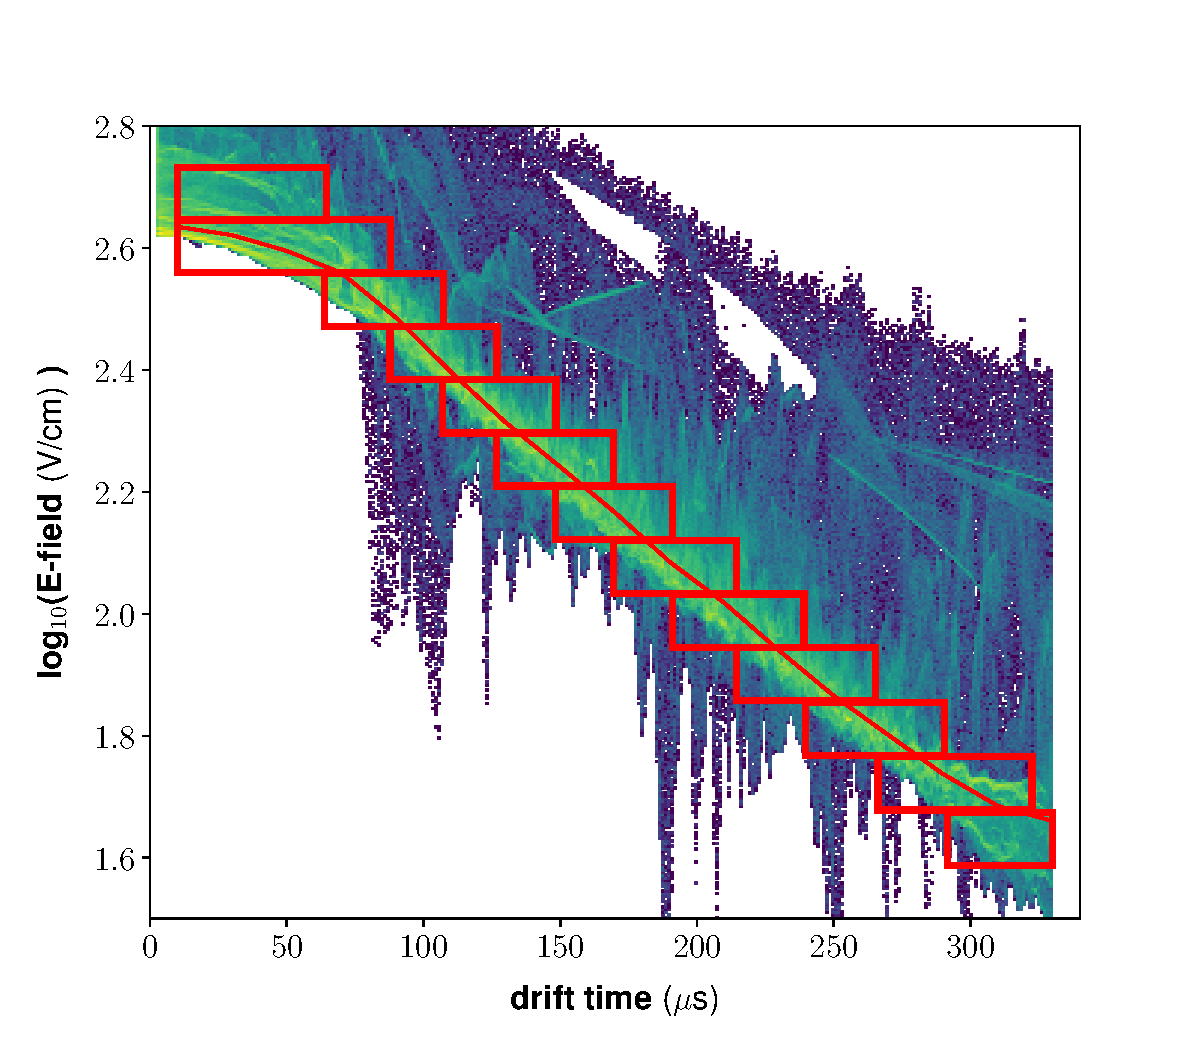
\includegraphics[width=\textwidth]{Figures/field_cut.pdf}
\caption{Electric field selection bins. } 
\label{fig:fieldbins}
\end{figure}

For any given drift time slice there will be a wide range of mapped field values. These will be near their minimum at the center of the detector and will increase dramatically as they approach the wall. Another way of saying this is that events in a given electric field slice will be drawn from a large range of drift times We would like to limit the range of drift times that events in an electric field slice, so we institute a further cut on our electric field bins. We find the overall trend in electric field by fitting a Gaussian to the electric field distribution in a series of drift time slices. We then interpolate between these fits to find a function, $F_{dT}(\mathcal{E}_{peak})$ which gives the drift time value associated with a given peak electric field. For each $i^{th}$ electric field bin we can now impose the following drift time cut:
\begin{equation}\label{eq:ebin_dt}
F_{dT}(1.1\cdot \mathcal{E}_{ctr,i}) < dT < F_{dT}(0.9\cdot \mathcal{E}_{ctr,i}) 
\end{equation}
\begin{table}
\centering
    \begin{tabular}{ c | c | c | c | c }
    \hline
    $\mathcal{E}_{ctr}$ & $dT_{min}$ & $dT_{max}$  & $\langle \mathcal{E} \rangle$ & $\sigma_{\mathcal{E}}$ \\ 
    \hline \hline
    43 & 291 & 330 & 43.2 & 2.5  \\
    \hline
    53 & 266 & 322 & 52.6 & 2.9  \\
    \hline
    65 & 240 & 290 & 64.8 & 3.7  \\
    \hline
    80 & 214 & 265 & 79.8 & 4.6  \\
    \hline
    98 & 191 & 239 & 97.8 & 5.6  \\
    \hline
    120 & 170 & 214 & 119.6 & 6.9  \\
    \hline
    147 & 148 & 191 & 146.7 & 8.3  \\
    \hline
    180 & 127 & 170 & 180 & 10  \\
    \hline
    220 & 107 & 148 & 219 & 13  \\
    \hline
    269 & 88 & 127 & 268 & 15  \\
    \hline
    329 & 64 & 107 & 329 & 19  \\
    \hline
    403 & 10 & 88 & 405 & 22  \\
    \hline
    491 & 10 & 65 & 484 & 28  \\ 
    \hline
    \hline
    \end{tabular}
    \caption{Selected electric field bin centers, along with the maximum and minimum drift time allowed for each bin. Also shown is the mean and standard deviation of electric fields for events in each bin.}
    \label{tan:fieldbins}
\end{table}

The selection of the various $\mathcal{E}_{ctr,i}$ began with the LUX Run03 average electric field of 180 V/cm. We then worked up in steps of 22.2\% and down in steps of 18.8\% to generate a set of non-overlapping bins that satisfied equation  \label{eq:ebin_e}. We do allow different bins to overlap in drift time, but the separation in field ensures that each bin is made up of an independent set of events. We did not include events above 10 microseconds or below 330 microseconds in drift time. The selected bins are shown in figure \ref{fig:fieldbins}, and the selected bin centers, along with the mean field value and its standard deviation is shown in table \ref{tab:fieldbins}.


\section{Argon-37 Non-Gaussianities}
Argon-37 provides three useful low-energy ER calibration lines. It decays through electron capture to $^{37}$Cl with a half life of 35 days. The long half life, combined with the fact that argon is chemically inert means that once injected, it will be on the order of a year before it has been sufficiently removed. That being the case, it was only injected immediately prior to LUX decommissioning\cite{ar371,pixey_ar37}.

The $^{37}$Ar source was produced through stimulated $\alpha$ emission of a $^{40}$Ca target using a neutron beam. The $^{37}$Ar sample used in LUX was produced by irradiating an aqueous solution of CaCl$_2$ with neutrons from an AmBe source. The gas above this solution was then collected and purified to obtain the gaseous sample of $^{37}$Ar\cite{pixey_ar37}. This sample was injected into the LUX xenon circulation using the same system as the $^{83m}$Kr calibrations\cite{lux_kr2}.

The three lines in the $^{37}$Ar decay are from the capture K-shell, L-shell, and M-shell electrons. The different captures have branching ratios of 0.9, 0.09, and 0.009 and will deposit x-rays with energies of 2.8224 keV, 0.2702 keV, and 0.0175 keV, respectively. The L-shell and M-shell captures are below the LUX threshold and so are of limited use to the work presented in this document. The K-capture x-ray will produce about 76 scintillation electrons, which will produce an S1 signal of about 6.7 phd. This is a small enough signal that there will be some non-Gaussian distortion in the S1 spectrum due to threshold effects. The charge yield for the K-capture is about 50 electrons/keV. With a 70\% extraction efficiency, there will be about 100 electrons extracted from an argon-37 event, which would produce an S2 of roughly 2500 phd assuming a single electron size of 25 phd. This is large enough that the S2 spectrum should be free of threshold effects.
\begin{figure}[h!]
\centering
\begin{subfigure}{0.5\textwidth}
  \centering
  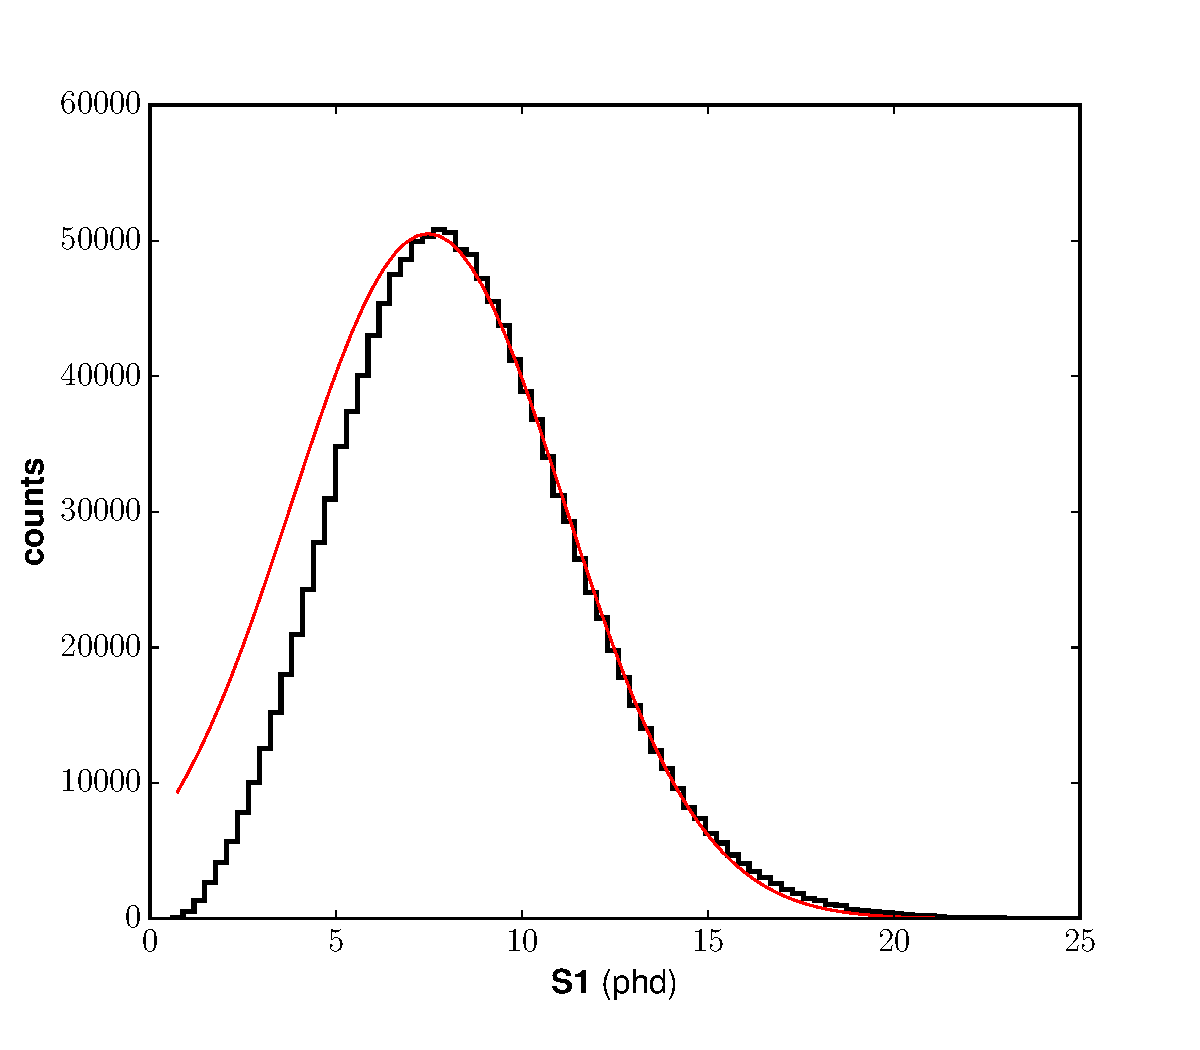
\includegraphics[width=\textwidth]{Figures/Ar37_S1spec.pdf}
  %\label{}
\end{subfigure}%
\begin{subfigure}{0.5\textwidth}
  \centering
  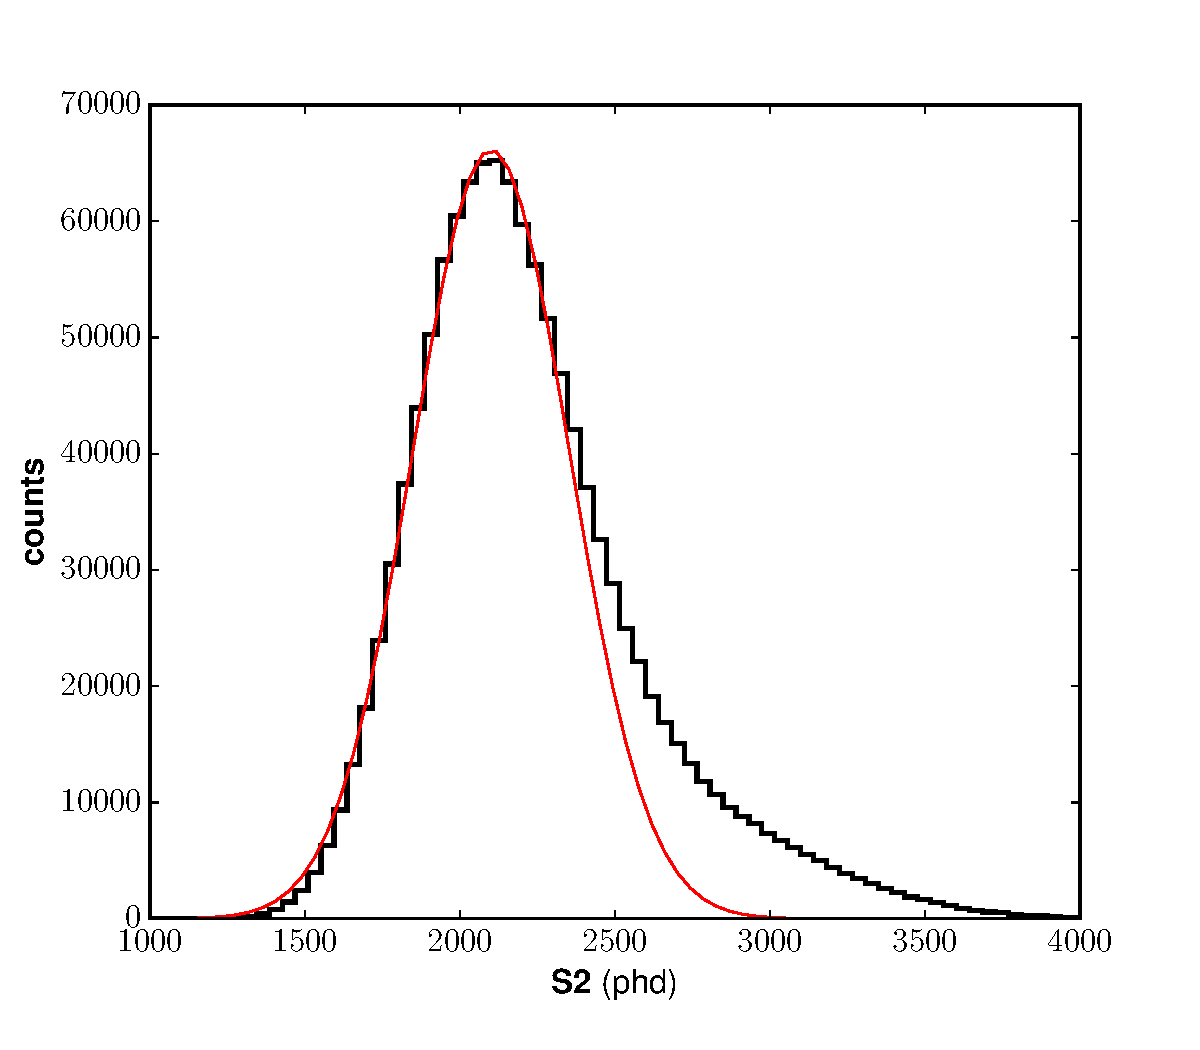
\includegraphics[width=\textwidth]{Figures/Ar37_S2spec.pdf}
  %\label{fig:intlin}
\end{subfigure}
\caption{The S1 and S2 spectra for the LUX $^{37}$Ar injection (black histograms), along with gaussian fits (red lines). Events with drift times between 105 and 170 $\mu$s. The S1 spectrum clearly does not behave like a gaussian on the low energy side of the spectrum. The S2 spectrum does have a  gaussian shape up until about 1 $\sigma$ above the mean at which point a pathological tail takes over. These S2 tails are a known issue and will be characterized in a later section.}
\label{fig:ddplot}
\end{figure}

The high rate and long lifetime of the argon-37 injection also meant that there was a huge number of events. From the injection on August 31$^{st}$ until the end of data-taking on September 3$^{rd}$ there were about 8.8 million argon-37 events. The fact that we have such a high-statistics dataset, combined with the spatially uniform nature of injection sources means that we can very finely probe the position-dependence of the detector response. This feature will be used to measure the S2 efficiency corrections and in defining our radial cut.


\section{Signal Corrections fo Post-Run04 Data}\label{sec:corrections}

\subsection{S2 Efficiency Correction from $^{37}$Ar}\label{sec:s2corr}
In Run4, the position-dependent efficiency corrections for the LUX S1 and S2 signals were obtained from a combination of tritium and $^{83m}$Kr calibration data. This method, which was described in section \ref{sec:krypcal}, relies in part on the fact that the S2 yields for small energy deposits have a minimal dependence on electric field. The first step in the KrypCal procedure is to measure the position dependence of the tritium peak S2 value. In order to derive the detector efficiency part of the position dependence, the field effect must first be removed. This field dependence is itself dependent on the energy of the events that contribute to the S2 peak. Since tritium is a beta spectrum, events with many energies will contribute to this peak, so an approximation is made that all of these events occur at 2.5 keV.

\begin{figure}[h!]
\centering
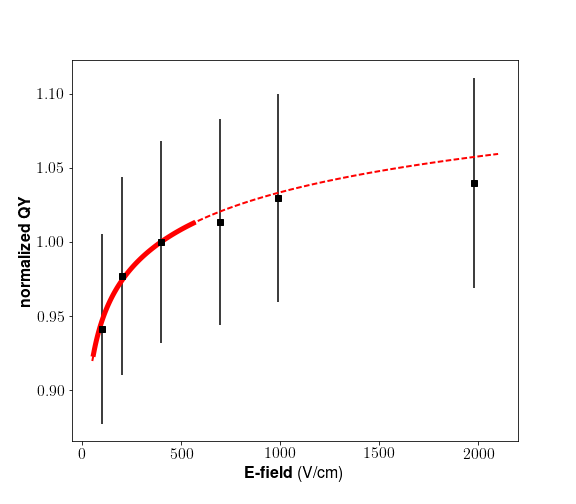
\includegraphics[width=150mm]{Figures/pixey_Ar_v_ef.png}
\caption{NEST model of the $^{37}$Ar vs the measurements from PIXeY\cite{pixey_ar37}. The solid portion of the line indicates the range of fields in the LUX post-Run4 calibration data. There is about a 10\% variation due to electric field in the LUX post-Run4 data. The NEST v0.98 model traces the trend in the PIXeY data quite well.}
\label{fig:pixey_Ar_v_ef} 
\end{figure}
It is here that we see a huge benefit in using the $^{37}$Ar K-capture peak instead of the tritium beta spectrum in deriving the S2. Because $^{37}$Ar is a mono-energetic line source rather than a continuous beta spectrum, we know that all of the events making up the S2 peak will come from a 2.8224 keV event, and no assumption or approximation need be made. 
\begin{figure}[h!]
\centering
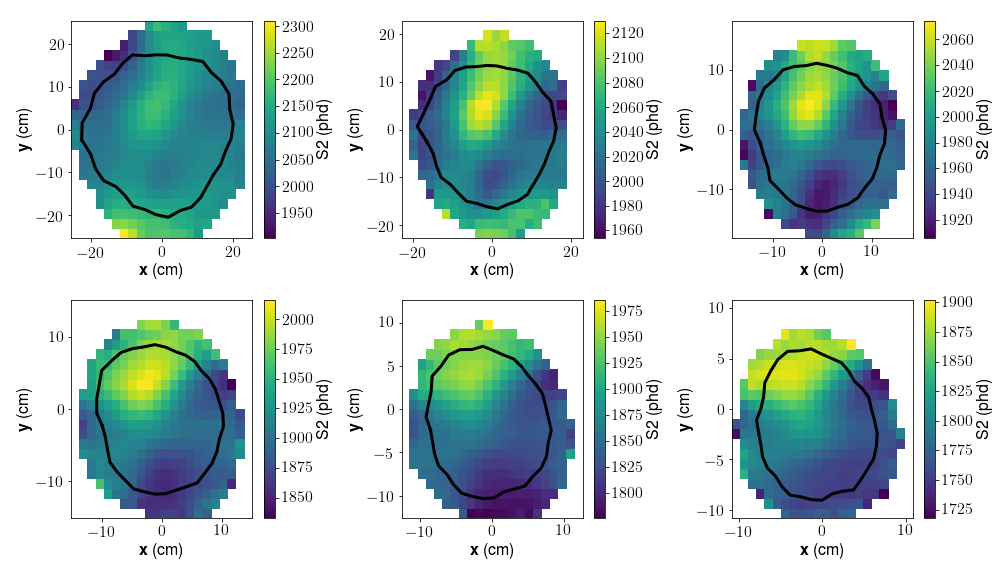
\includegraphics[width=150mm]{Figures/S2map_xy.png}
\caption{Measured Ar-37 S2 means in selected drift time bins. The bins from top left to bottom right are 50, 100, 150, 200, 250, and 300 microseconds. The black outline indicates the x-y position of the radial selection cut at the given drift time. The measurements of the S2 mean outside of this border exist because of the smearing applied in the calculation. }
\label{fig:S2map_xy} 
\end{figure}

The first step is to divide the detector into bins of 10 microseconds. We set the highest drift time bin edge to be at 5 microseconds, which is the approximate position of the gate grid. The lowest bin edge is set to 485 microseconds, although our analysis will only include events above 330 microseconds in drift time, which corresponds to the bottom of the detector at x=y=0 cm.
\begin{figure}[h!]
\centering
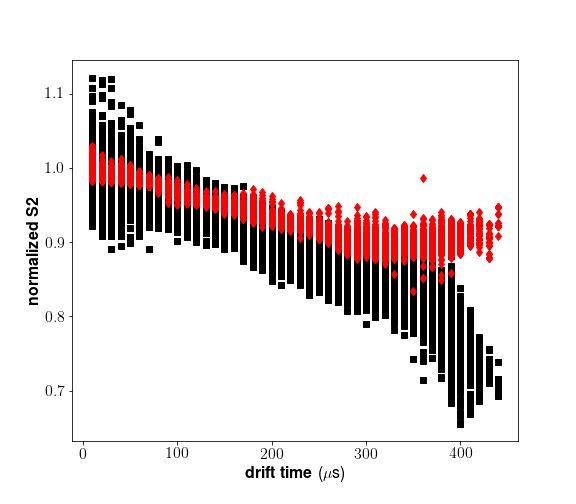
\includegraphics[width=150mm]{Figures/S2trend_dt.png}
\caption{The black markers here show the measured S2 means, normalized to the top center of the detector. The red markers show the expected variation due to electric field alone. The S2 efficiency correction can be thought of as the red values divided by the black values.}
\label{fig:S2trend_dt} 
\end{figure}

Each drift time bin is then divided into a 22x22 x-y grid. The radial extent of events is highly dependent on drift time, so the density in x and y of events near the top of the detector is much less than the density near the bottom of the detector. Events from the bottom of the detector are focused from about 25 cm in real space to about 9 cm in S2 space. This means that the S2 from a wall event (25 cm radius) near the bottom of the detector will appear to have a radius of about 10 cm. An x-y bin with edge-width of 2 cm at the top of the detector will have an effective width of about 5 cm at the bottom of the detector. To account for these effects, we scale the x-y grid for each drift bin by the maximum radius of events within that bin. The 10 microsecond drift bin has an x-y grid that spans from -25.2 to 25.2 cm, while the 330 microsecond grid goes from -9.4 to 9.4 cm.

\begin{figure}[h!]
\centering
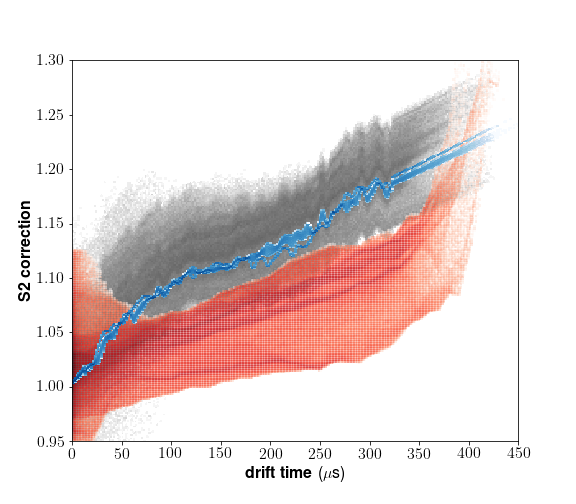
\includegraphics[width=150mm]{Figures/S2corr_dt.png}
\caption{The KrypCal z-only (blue) and xyz (grey) S2 corrections compared to the Ar-37 S2 correction (red). At drift times greater than about 100 microseconds the two methods are in decent agreement. At smaller drift times, however, there is a steep trend observed in KrypCal that is not present in the corrections measured using Ar-37.}
\label{fig:S2corr_dt} 
\end{figure}
When calculating the mean values, we treat the drift time bins independently but allow the x-y bins to smear together. We draw a circle with a radius equal to 2.5 times the bin width around the center of each  x-y bin. We include all of the events within that circle in our calculations for that bin. For each bin we calculate the mean S2 ($S2_{H3,ijk}$), where $i$ is the x-index, $j$ is the y-index, and $k$ is the drift time index, as well as the mean electric field using values interpolated from a field-map described in section \ref{sec:efield}. The electric field value is used to generate an expected S2 value from NEST, ($S2_{NEST,ijk}$).

\begin{figure}[h!]
\centering
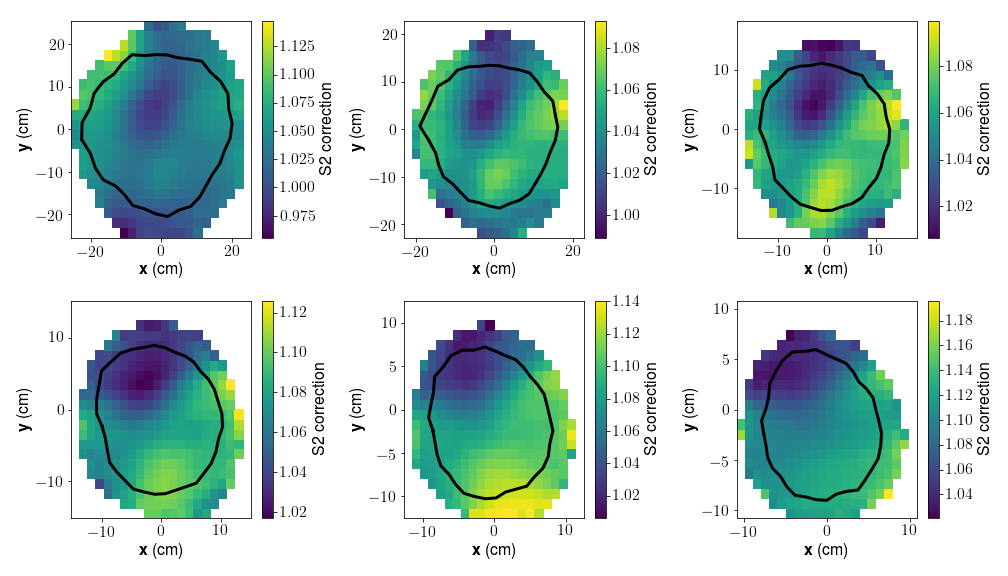
\includegraphics[width=150mm]{Figures/S2corr_xy.png}
\caption{Measured S2 corrections for the same drift time bins as in figure \ref{fig:S2map_xy}. }
\label{fig:S2corr_xy} 
\end{figure}
The S2 measurements need to be normalized to the top center of the detector. We calculate the S2 value in this region by taking the average of bins from the top three drift time slices that lie inside a radius of 10 cm from the center of the detector. The S2 correction is then defined:
\begin{equation}
C_{S2,ijk}=\frac{S2_{NEST,ijk}}{S2_{H3,ijk}}\cdot \frac{S2_{H3,top}}{S2_{NEST,top}},
\end{equation}
where $S2_{NEST,top}$ and $S2_{H3,top}$ are the values calculated at the center top of the detector.

Figure \ref{fig:S2corr_dt} shows a comparison of the S2 corrections measured using the procedure described in this section and those measured using the KrypCal procedure. Below about 100 microseconds in drift time, the slope from the two corrections methods are in good agreement. For drift times less than 100 microseconds, the KrypCal corrections see a significantly larger slope than those measured using argon-37. There are fewer assumptions that go into the argon-37 S2 corrections. In particular, the assumption that the peak of the tritium spectrum can be approximated by a mono-energetic peak has the potential to introduce systematic effects. A change in the electric field may induce enough of a change to the charge and light yields that the energy of events in the peak of the tritium S2 spectrum is dependent on electric field. 

We test this by looking at simulated tritium events which were generated using charge and light yields which will be presented in the next chapter. We take the mean input energy of events in a 200 phd window centered on the maximum of the uncorrected S2 spectrum. At the top of the detector, where electric field equals 491 V/cm, the energy of events in the peak of the S2 spectrum is 4.0 keV. At the bottom of the detector where the electric field is 43 V/cm, the energy of the S2 peak is 20\% higher at 4.8 keV. At these energies, the charge yield has a steep dependence with energy, so there will likely be non-negligible systematic effects introduced by assuming the tritium S2 dependence can be approximated using a constant energy. This clearly highlights the advantage of using the mono-energetic Ar-37 peak to measure the S2 position-dependent efficiency.

\subsection{S1 corrections from Xenon-131m + Krypton-83m Doke Plot}\label{sec:s1dokeplot}
In a detector with a non-uniform electric field, the S1 efficiency correction is more complicated to measure than the S2 correction. In order to limit the effects of electric field variation, we would like to use a low-energy calibration source because the field dependence of charge and light yields is smallest at low energies. This is also the energy scale with the lowest light yield and combined with the typically low light-collection efficiency of liquid xenon TPC's (roughly 9-10\% for LUX), these low-energy sources suffer from threshold effects in their S1 spectra. The KrypCal procedure feeds the S2 efficiency correction measured using tritium data into the krypton-83m S2 spectrum. This yields a field-dependent S2 spectrum which is used to measure the position-dependent recombination of krypton-83m data. This recombination measurement is then fed into the krypton-83m S1 spectrum in order to get a measurement of the S1 position-dependent efficiency.

Here we test an alternate method for measuring the S1 efficiency corrections which utilizes both the xenon-131m and krypton-83m calibration data. This method takes advantage of the fact that the field dependence of the charge and light yields is completely contained in the recombination probability. This means that when the data is plotted on a Doke-style plot, variation in the electric field will only work to move points along a line and will not change the line's parameters. The aim of this method, then, is to use a Doke-style plot to directly measure the light correction efficiency (G1) in each of our (x, y, dT) bins which were described in the previous section. This method relies on the same recombination model the KrypCal assumes but, unlike KrypCal, does not require prior knowledge of the initial exciton to ion ratio, $\alpha$.
\begin{figure}[h!]
\centering
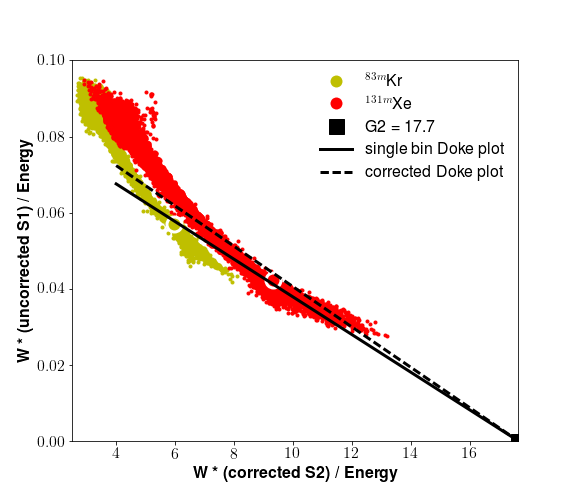
\includegraphics[width=150mm]{Figures/S1corr_singlebin.png}
\caption{Doke plots of xenon-131m and krypton-83m for the bins described in section \ref{sec:s2corr}. By forcing G2 to be constant, we perform a single-parameter fit to find G1 in each bin. The solid black line shows the best fit line for the selected bin, and the dashed line represents G1, G2 as measured at the center of the detector.  }
\label{fig:S1corr_singlebin} 
\end{figure}

We use the same method to measure the krypton-83m and xenon-131m S1 and S2 means for each voxel as was used in section \ref{sec:s2corr} to measure the S2 means of argon-37. Once these means ($S1_{Kr83m,ijk}$, $S1_{Xe131m,ijk}$, $S2_{Kr83m,ijk}$, and $S2_{Xe131m,ijk}$) have been measured, we use them to measure G1 and G2 at the center of the detector. We define the center of the detector as the mean drift time of argon-37 events, which is calculated to be 162.2 microseconds. We select bins that are within 20 microseconds drift time of the detector center and have a radius less than 5 cm. We take the average of the uncorrected S1 values, and the average of the corrected S2 values ($S2_{ijk}\cdot C_{S2,ijk}$). We then construct our Doke-plot using:
\begin{equation}
\begin{split}
X_{center}=& W\cdot S2_{center}\cdot C_{S2,center}/E\\
Y_{center}=& W\cdot S1_{center}/E,
\end{split}
\end{equation}
where $W=1/73$ is the average work function for ionization and scintillation in liquid xenon, and $E$ is the energy of the calibration line. We draw a line through the points ($X_{Xe131m,center},Y_{Xe131m,center}$) and ($X_{Kr83m,center},Y_{Kr83m,center}$). The x-intercept of this line will be taken to be G2$_{center}$, and the y-intercept will be G1$_{center}$.
\begin{figure}[h!]
\centering
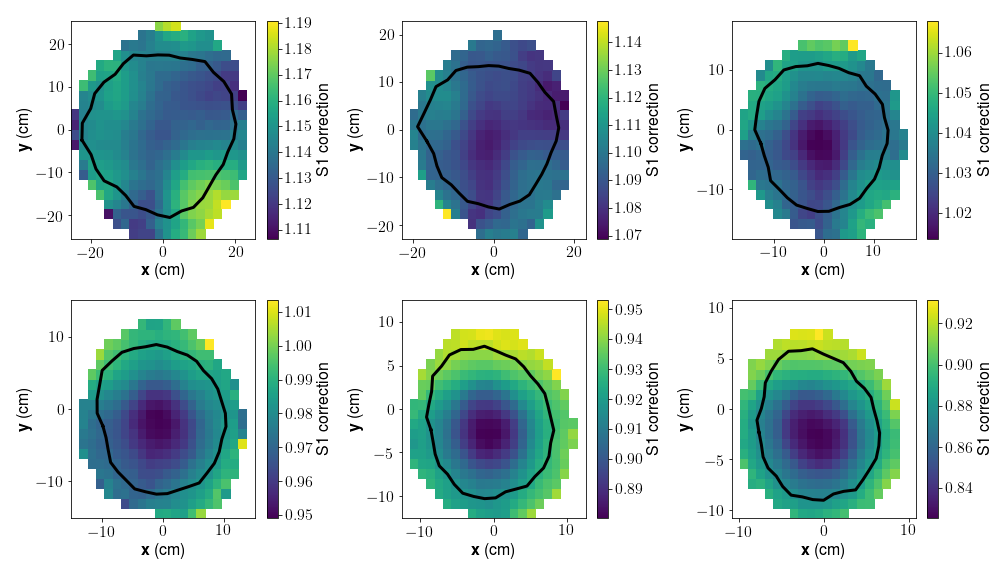
\includegraphics[width=150mm]{Figures/S1corr_xy.png}
\caption{Measured S1 corrections for the same selected drift time bins as in figure \ref{fig:S2map_xy}. }
\label{fig:S1corr_xy} 
\end{figure}


The value of G1 for the individual voxels is calculated in the same manner as was done for the detector center. We define the points ($X_{ijk},Y_{ijk}$) for krypton-83m and xenon-131m in the same way we defined ($X_{center},Y_{center}$). Here, instead of analytically drawing a line through the two points, we fix the x-intercept to G2$_{center}$ and allow the y-intercept to float in order to find the best-fit G1$_{ijk}$. These values of G1$_{ijk}$ are direct measurements of the position-dependent S1 efficiency, so by normalizing them to the detector center we can easily write the S1 efficiency correction:
\begin{equation}
C_{S1,ijk}=\frac{G1_{center}}{G1_{ijk}}
\end{equation}
\begin{figure}[h!]
\centering
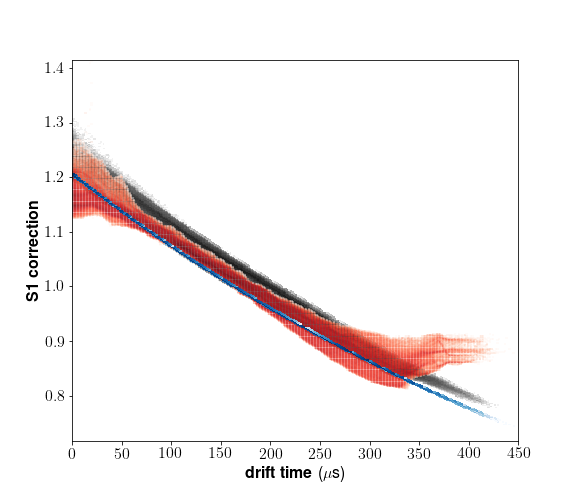
\includegraphics[width=150mm]{Figures/S1corr_dt.png}
\caption{Comparison of the KrypCal z-only (blue) and xyz (grey) S1 corrections with the Doke-style S1 corrections introduced in this section (red). }
\label{fig:S1corr_dt} 
\end{figure}

This method of deriving the S1 efficiency correction is more consistent with KrypCal than the argon-37 S2 corrections were. This is more or less expected, since the two methods rely on the same physical assumption. The primary discrepancy between the two would be expected to come from the fact that both methods require the S2 correction as an input.The roughly 5\% discrepancy in the S2 correction is subdominant to both the variation in both recombination and S1 efficiency, so it has only a minor effect on the measurement of the S1 correction.  

\subsection{Applied Corrections}
Now that we have measured a new set of corrections we would like to apply them to our data in order to see how they compare to the existing KrypCal corrections. To do this we need to interpolate between the measured $C_{S2,ijk}$ and $C{S1,ijk}$ to find a set of corrections for arbitrary x, y, and dT.
\begin{figure}[h!]
\centering
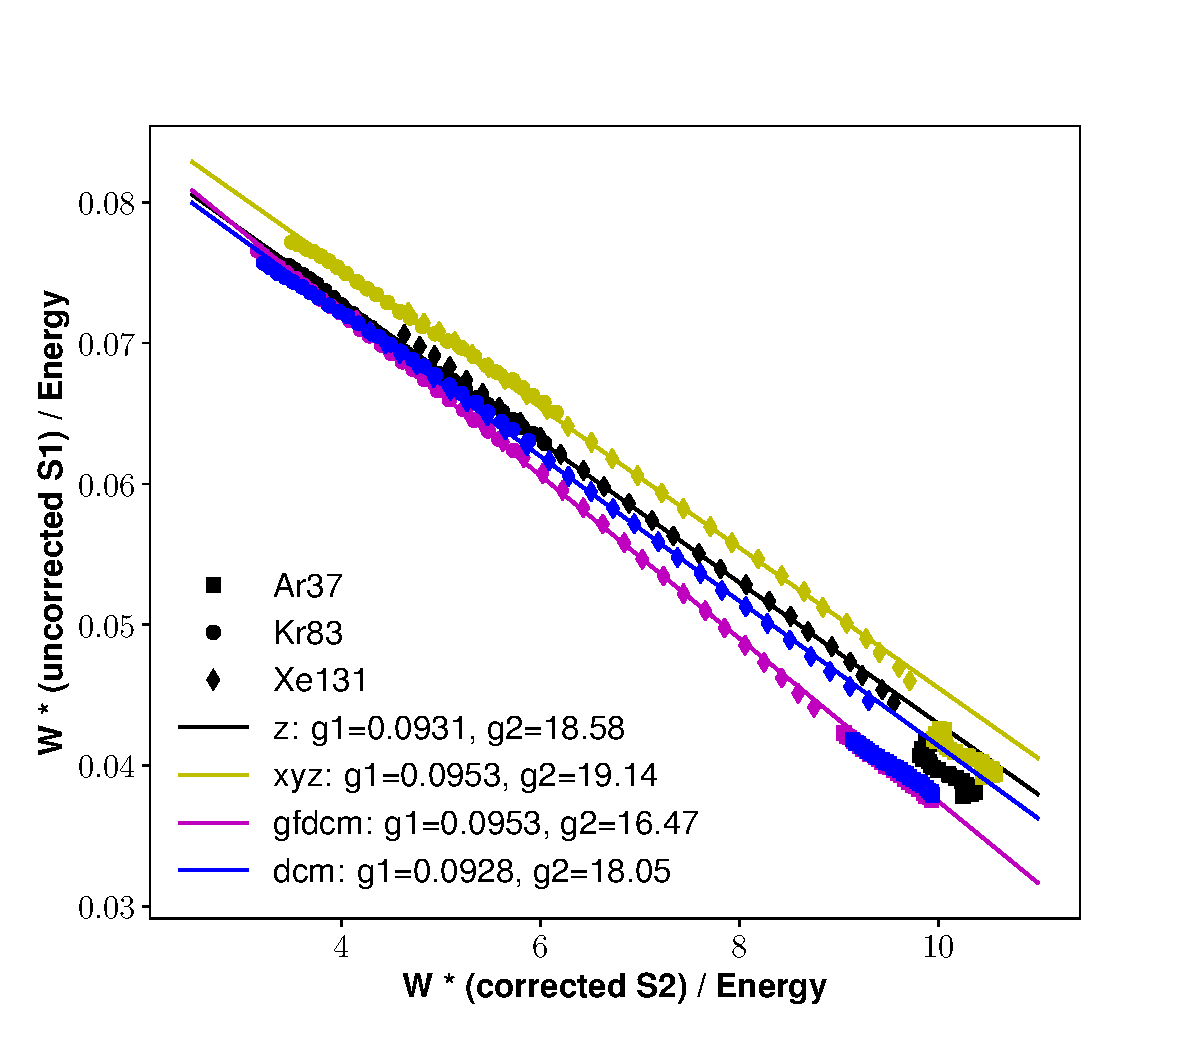
\includegraphics[width=150mm]{Figures/dt_doke_plot.pdf}
\caption{Doke-style plot for the various corrections methods considered. See text for explanation of the various lines.}
\label{fig:dt_doke_plot} 
\end{figure}

In order to ensure that there is no out-of-bounds interpolation error, we set the corrections values of any empty bins equal to that of their nearest non-empty neighbor. For each drift time bin we apply a bivariate spline in x and y, taking $C_{S2,ijk}$ and $C{S1,ijk}$ to be located at the center of their respective bins. After that we apply a linear interpolation in drift time between the values of the x-y splines. Again we assume the values are located at the centers of their respective drift time bins.

With the newly corrected data in hand, we now check to see how we did. We first need to measure the final G1 and G2 for both types of corrections to do this we finely slice the detector in drift time and generate a Doke-style plot using the same procedure as in the previous section. This time we include the krypton-83m and xenon-131m points from all of the drift time slices when fitting our line, and we allow both G1 and G2 to float. We do not include the argon-37 point in the fit because they are too close to threshold and are not expected to lie on the Doke-plot line. 
\begin{figure}[h!]
\centering
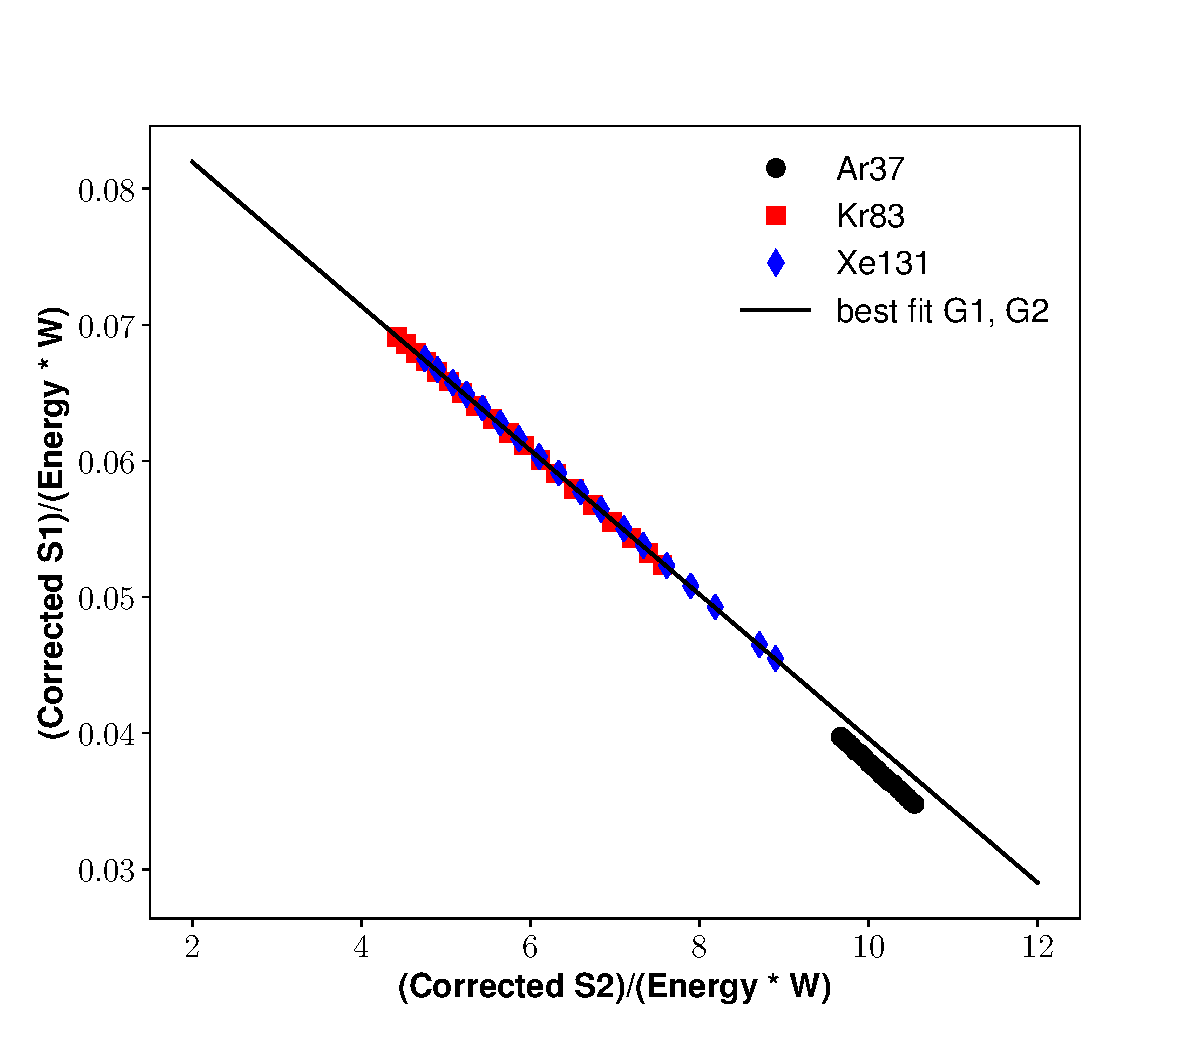
\includegraphics[width=150mm]{Figures/NEST_g1g2_dcm.pdf}
\caption{Simulated version of figure \ref{fig:dt_doke_plot} generated using the libNEST code. We set G1=0.0928 and G2=17.49 in this plot. This plot was generated without the model of the S2 tail, which will be introduced in the next section.}
\label{fig:dt_doke_plot_libnest} 
\end{figure}

The results of these fits are shown in figure \ref{fig:dt_doke_plot}. In this plot the lines labeled ``z'' and ``xyz'' are KrypCal corrections. The line labeled ``dcm'' is using the corrections derived in the previous two sections. The ``dc'' in ``dcm'' is shorthand for ``Doke-corrected'', and the ``m'' indicates that the S1 and S2 averages in the various bins were calculated by arithmetic mean. We also generated a set of corrections which fit a Gaussian peak to the S1 and S2 distributions in the individual bins, but the two methods yielded equivalent results, so we discarded the latter for the sake of simplicity. The newly derived corrections do improve the fit to a Doke line. The rms offset of the fitting points from their best fit lines is 5.6\% and 5.2\% for ``z'' and ``xyz'', respectively, and is 4.3\% for both ``dcm'' and ``gfdcm''. This improvement indicates that the corrections method laid out in the previous sections does a better job at flattening out the position dependence of the detector efficiency.
\begin{figure}[h!]
  \centering
  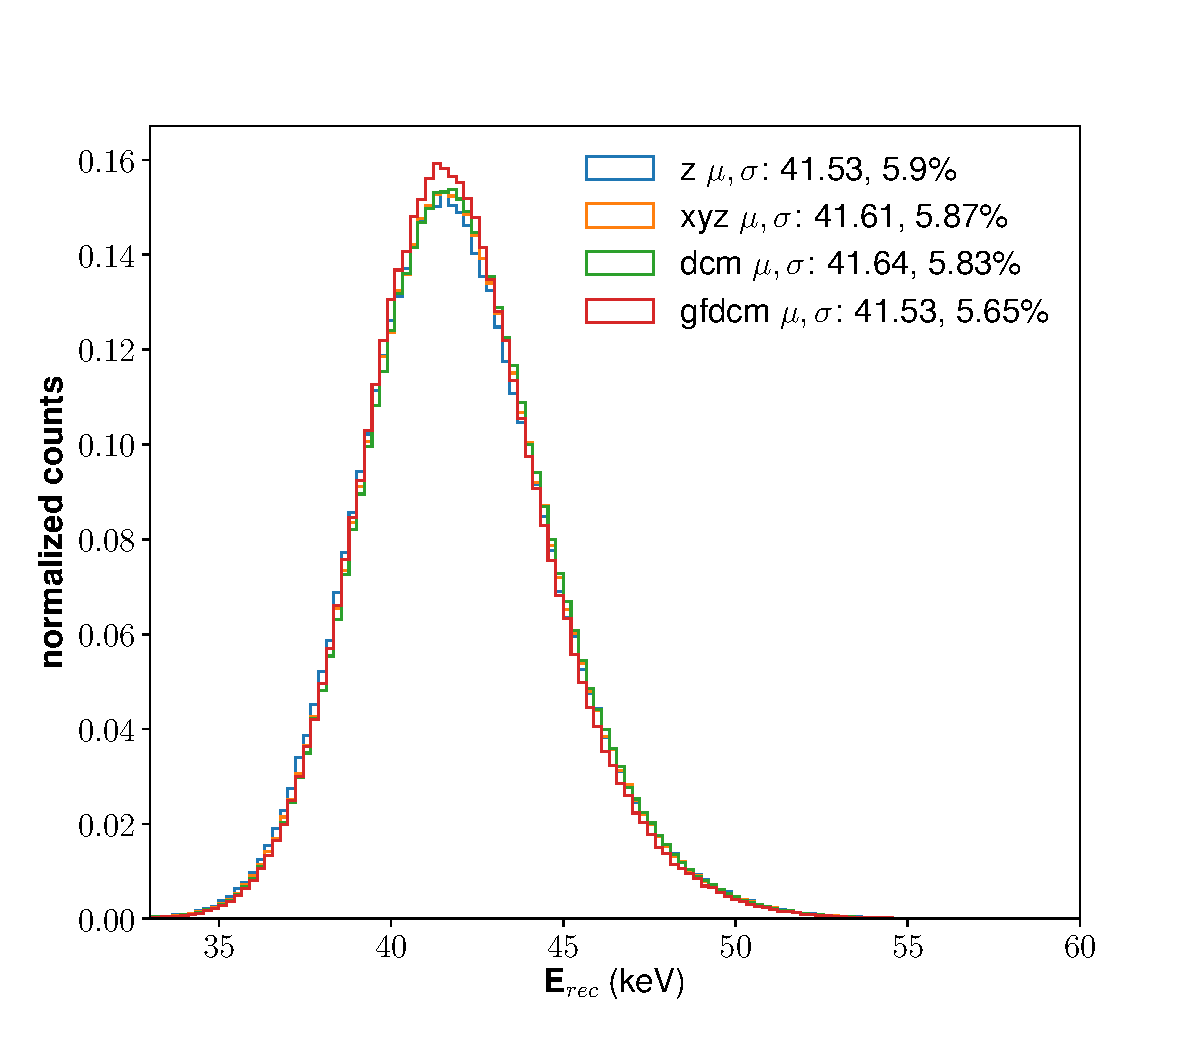
\includegraphics[width=\textwidth]{Figures/E_spec_Kr.pdf}
  \caption{Reconstructed energy spectrum for the 41.5 keV krypton-83m spectrum. The $\mu$ indicates the peak location and is in units of keV. $\sigma$ indicates the width/energy of the spectrum.}
\label{fig:E_spec_Kr} 
\end{figure}

Figure \ref{fig:dt_doke_plot_libnest} shows a simulation of the plots in figure \ref{fig:dt_doke_plot}. The G1 and G2 values used for this simulation were G1=0.0928 and G2=17.49. The best-fit line in \ref{fig:dt_doke_plot_libnest} is able to reproduce these values within about 0.1\%, yielding G1=0.0926 $\pm0.0001$, and G2=17.48 $\pm0.04$. The measured G1 is off of the true value by about 2-sigma; this is likely due to a small systematic effect in the libNEST code. This 0.1\% effect is is highly subdominant to other uncertainties in our measurements, so we will neglect it. The argon-37 K-capture points are systematically below the best fit line by, on average 4.5\%. For comparison, the argon-37 points in figure \ref{fig:dt_doke_plot} are below their best fit lines by 8\% for ``z'' corrections, 1\% for ``gfdcm'' corrections, and 9\% for ``dcm'' corrections. 
\begin{figure}[h!]
\centering
  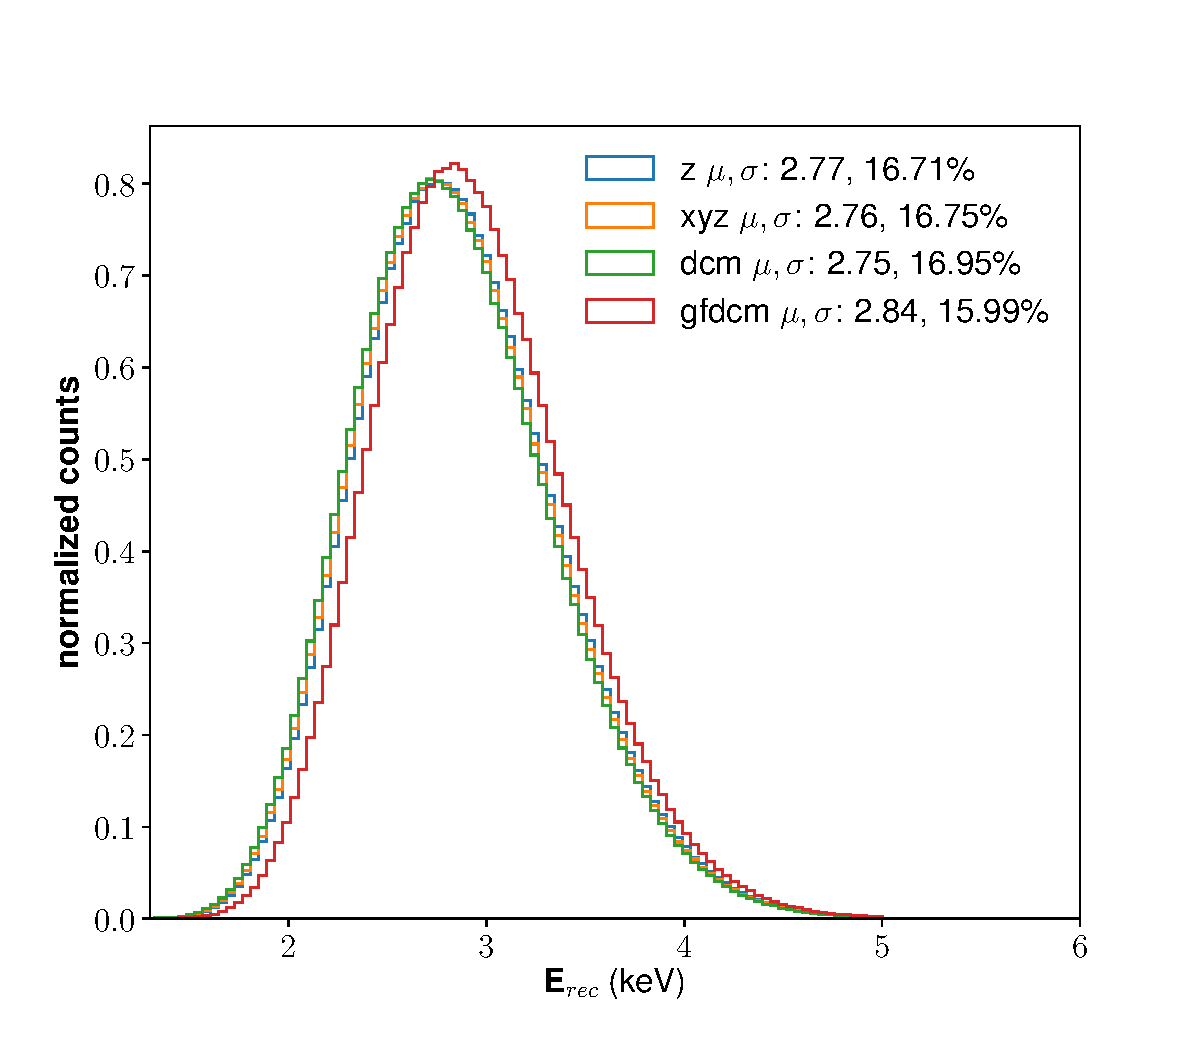
\includegraphics[width=\textwidth]{Figures/E_spec_Ar.pdf}
  \caption{Reconstructed energy spectrum for the 2.8224 keV argon-37 spectrum. The $\mu$ indicates the peak location and is in units of keV. $\sigma$ indicates the width/energy of the spectrum.}
\label{fig:E_spec_Ar} 
\end{figure}

The line in figure \ref{fig:dt_doke_plot} labeled ``gfdcm'' also uses the corrections derived in the previous two sections. The difference between this data and the ``dcm'' data is that it uses a different measure of S2. The ``dcm'' data, along with ``z'' and ``xyz'', uses the ``pulse-finder'' area as the measure of S2. This is just a raw sum of the S2 waveform. The ``gfdcm'' data uses the area under a Gaussian function (hence the ``gf'') which has been fit to the S2 waveform as the measure of S2 size.   
\begin{figure}[h!]
  \centering
  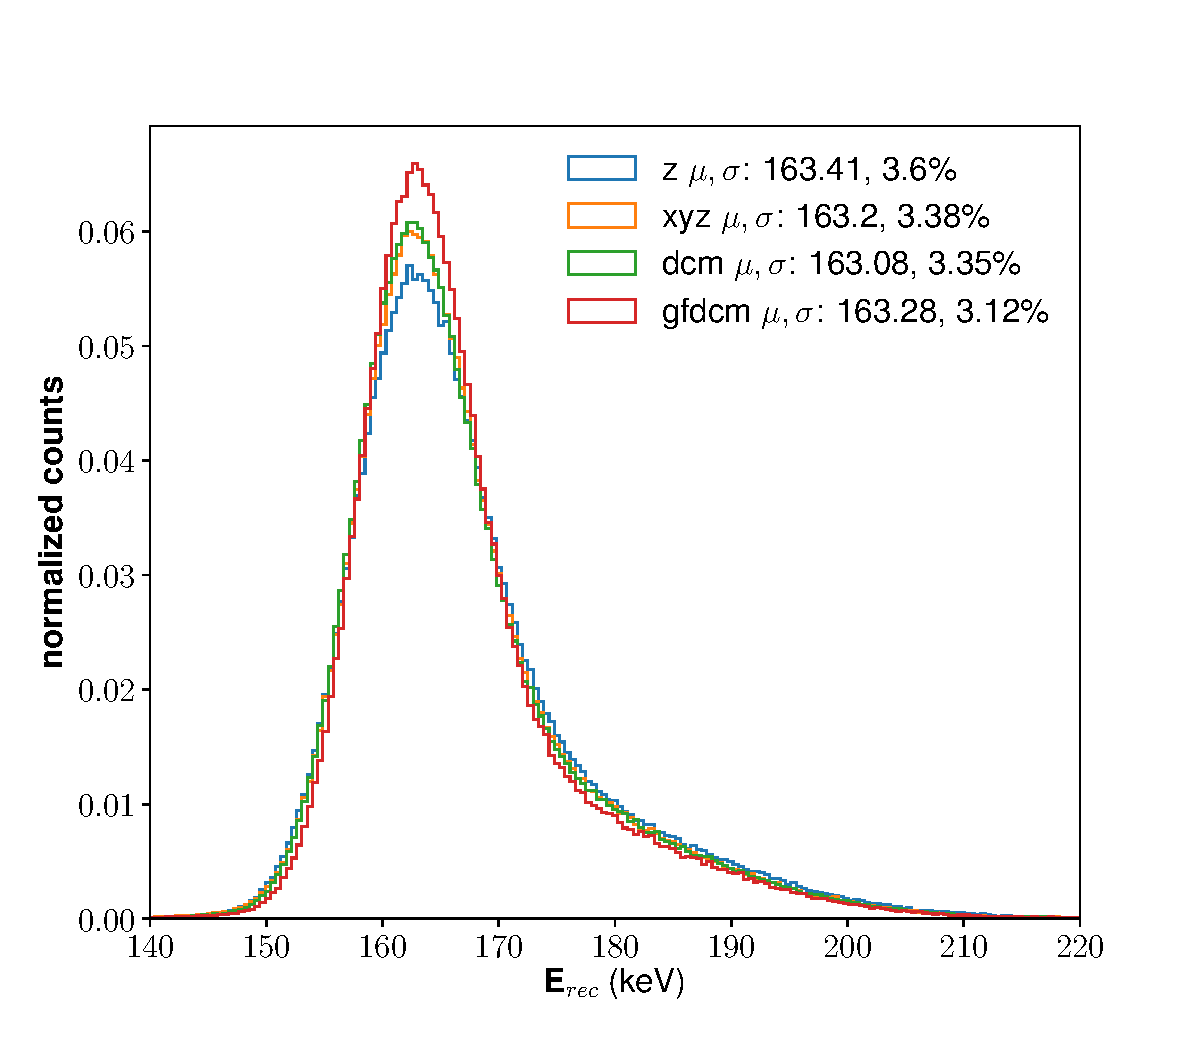
\includegraphics[width=\textwidth]{Figures/E_spec_Xe.pdf}
  \caption{Reconstructed energy spectrum for the 163.93 keV xenon-131m spectrum. The $\mu$ indicates the peak location and is in units of keV. $\sigma$ indicates the width/energy of the spectrum.}
\label{fig:E_spec_Xe} 
\end{figure}

The first observation we take from figure \ref{fig:dt_doke_plot} is that there is a systematic variation in the argon-37 points, causing them to be ``S'' shaped. Thiseffect is not present in the ``dcm'' of ``gfdcm'' plots, and so provides further evidence that the steep trend in the KrypCal S2 correction near the top of the detector does not represent a genuine efficiency effect. The argon-37 populations in the ``z'', ``xyz'', and ``dcm'' plots are also offset from the best fit line. This is not entirely unexpected since the argon-37 S1 spectrum is bumping against threshold, although the size of the offset is larger than expected.

We use the G1 and G2 values taken from to generate reconstructed energy spectra for xenon-131m, krypton-83m, and argon-37. We find that ``z'', ``xyz'', and ``dcm'' generate a roughly equivalent energy spectrum for argon-37 and krypton-83m, both in the peak location and resolution. For xenon-131m, ``dcm'' and ``xyz'' are roughly equivalent and ``z'' produces a spectrum which is wider by about 7.5\%. 

Interestingly, the ``gfdcm'' corrections produce significantly narrower spectra than any of the others, for all three calibration lines. Additionally, it produces the only argon-37 spectrum whose energy is higher than the true value of 2.8224 keV. This is important because the reconstructed energy for argon-37 should be artificially high because the low energy side of the spectrum is hidden by threshold. TMoving forward, we will focus on the following three corrections methods: 
\begin{itemize}
\item ``dcm'', because it produces ever-so-slightly better Doke plot and energy spectra than ``z'' and ``xyz''
\item ``gfdcm'', because it produces the straightest Doke-plot and best energy spectra out of any of the methods tested
\item ``z'', in order to be consistent with, and to create applicable results for existing LUX analysis
\end{itemize}



\section{Model of the Pathological S2 Tails}\label{sec:s2tails}
The energy spectra shown in figures \ref{fig:E_spec_Ar}, \ref{fig:E_spec_Kr}, and \ref{fig:E_spec_Xe} all have a clear non-Gaussian tail toward high energy. These tails stem from a pathological effect in the S2 signals. Their physical root is not clear, although there is some evidence that they are at least in part caused by trains of un-extracted electrons from previous events which are emitted from the liquid surface over a millisecond time scale. Regardless of their origin, the S2 tails are present both during the LUX Run04 WIMP-search and in the post-Run04 calibration campaign. In this section we will develop a purely empirical model of the tails in order to reproduce the shapes of the S2 and reconstructed energy spectra.

We look for insight into this issue by comparing the S2 spectra of argon-37, xenon-131m, and krypton-83m at different drift times, as in figure \ref{fig:E_spec_tails}. We find that the relative amplitude and slope of the tails do not change significantly at different energies or drift bins. From this we conclude that the tails will be approximately proportional to the initial S2 size. This is good news because it means that the combined energy model presented in section \ref{sec:nest} will still be expected to hold. We also see from figure \ref{fig:E_spec_tails_ar} that the shape and size of the argon-37 tails do not change when additional activity, in the form of krypton-83m events, is added to the detector.
\begin{figure}[h!]
  \centering
  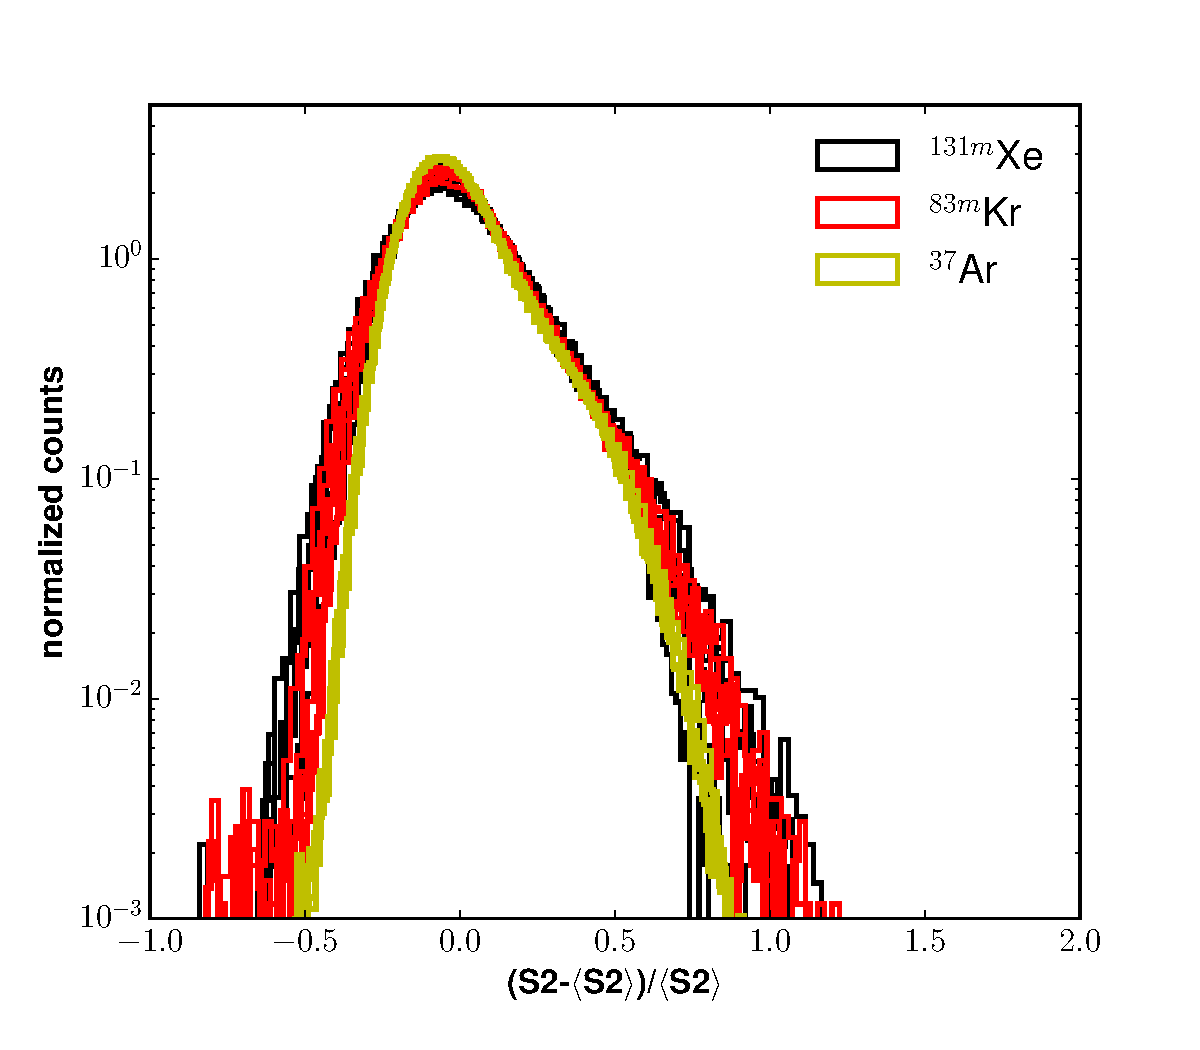
\includegraphics[width=\textwidth]{Figures/S2_tail_spec_all.pdf}
  \caption{Mean-subtracted and normalized S2 spectra for argon-37, krypton-83m, and xenon-131m. The spectra are divided into 6 drift time bins from 40 to 310 microseconds. We see in this plot that the fractional size of the S2 tails is roughly constant in both energy and drift time.}
\label{fig:E_spec_tails} 
\end{figure}

To first order, the effect of the pathological tails will be absorbed into the measurement of G2. In calculations where the detector resolution are important, such as in the measurement of recombination fluctuations or when dealing with continuous energy spectra, a more nuanced understanding may be required. To this end, we aim to develop an empirical model which will allow us to estimate the systematic effects of this pathology.
\begin{figure}[h!]
  \centering
  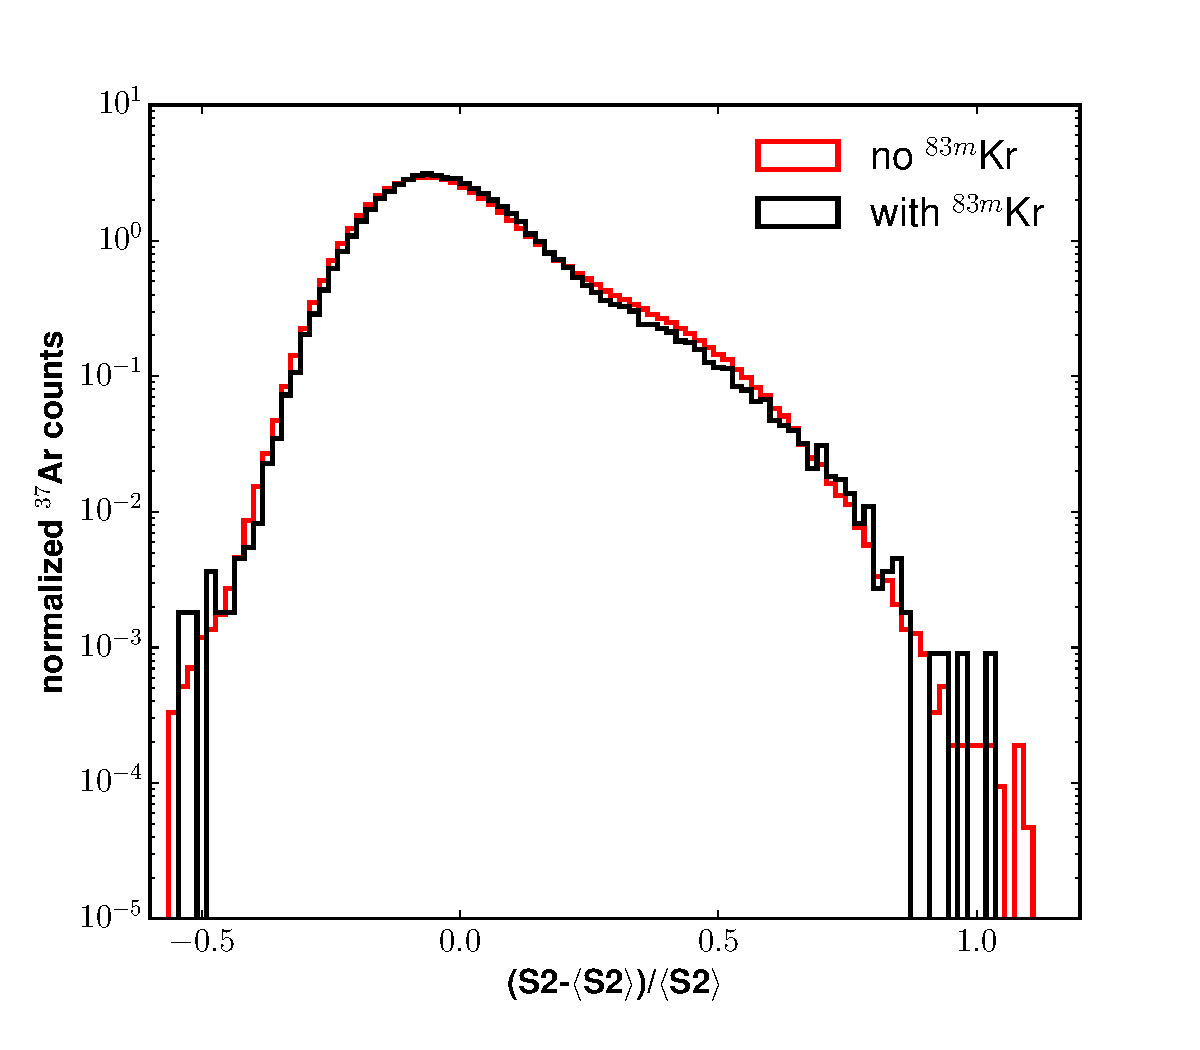
\includegraphics[width=\textwidth]{Figures/S2_tail_spec_Ar_rate.pdf}
  \caption{Mean-subtracted and normalized S2 spectra for argon-37. We show the spectrum both during a krypton-83m calibration (black), and when no additional activity is present (red).}
\label{fig:E_spec_tails_ar} 
\end{figure}

The model of S2 tails will be implemented as an adjustment to the libNEST model by adding some random number of electrons to number of electrons extracted from the liquid. The expected value for the number of extracted electrons before the tail is added is given by:
\begin{equation}
\langle N_{e,extr} \rangle = \epsilon N_{e} /C_{S2}(x,y,dT),
\end{equation}
where $\epsilon$ is the extraction efficiency, $C_{S2}(x,y,dT)$ is the efficiency correction for the event, and $N_e$ is the number of electrons generated in the liquid. To simulate the effect of the S2 tails, we will alter $N_{e,extr}$ to give $N'_{e,extr}$, which will then continue to propagate through the libNEST model as usual. The resulting S2 spectra generated will hopefully reproduce the shape of the S2 spectra we observe in data.


\begin{figure}[h!]
\centering
\begin{subfigure}{0.5\textwidth}
  \centering
  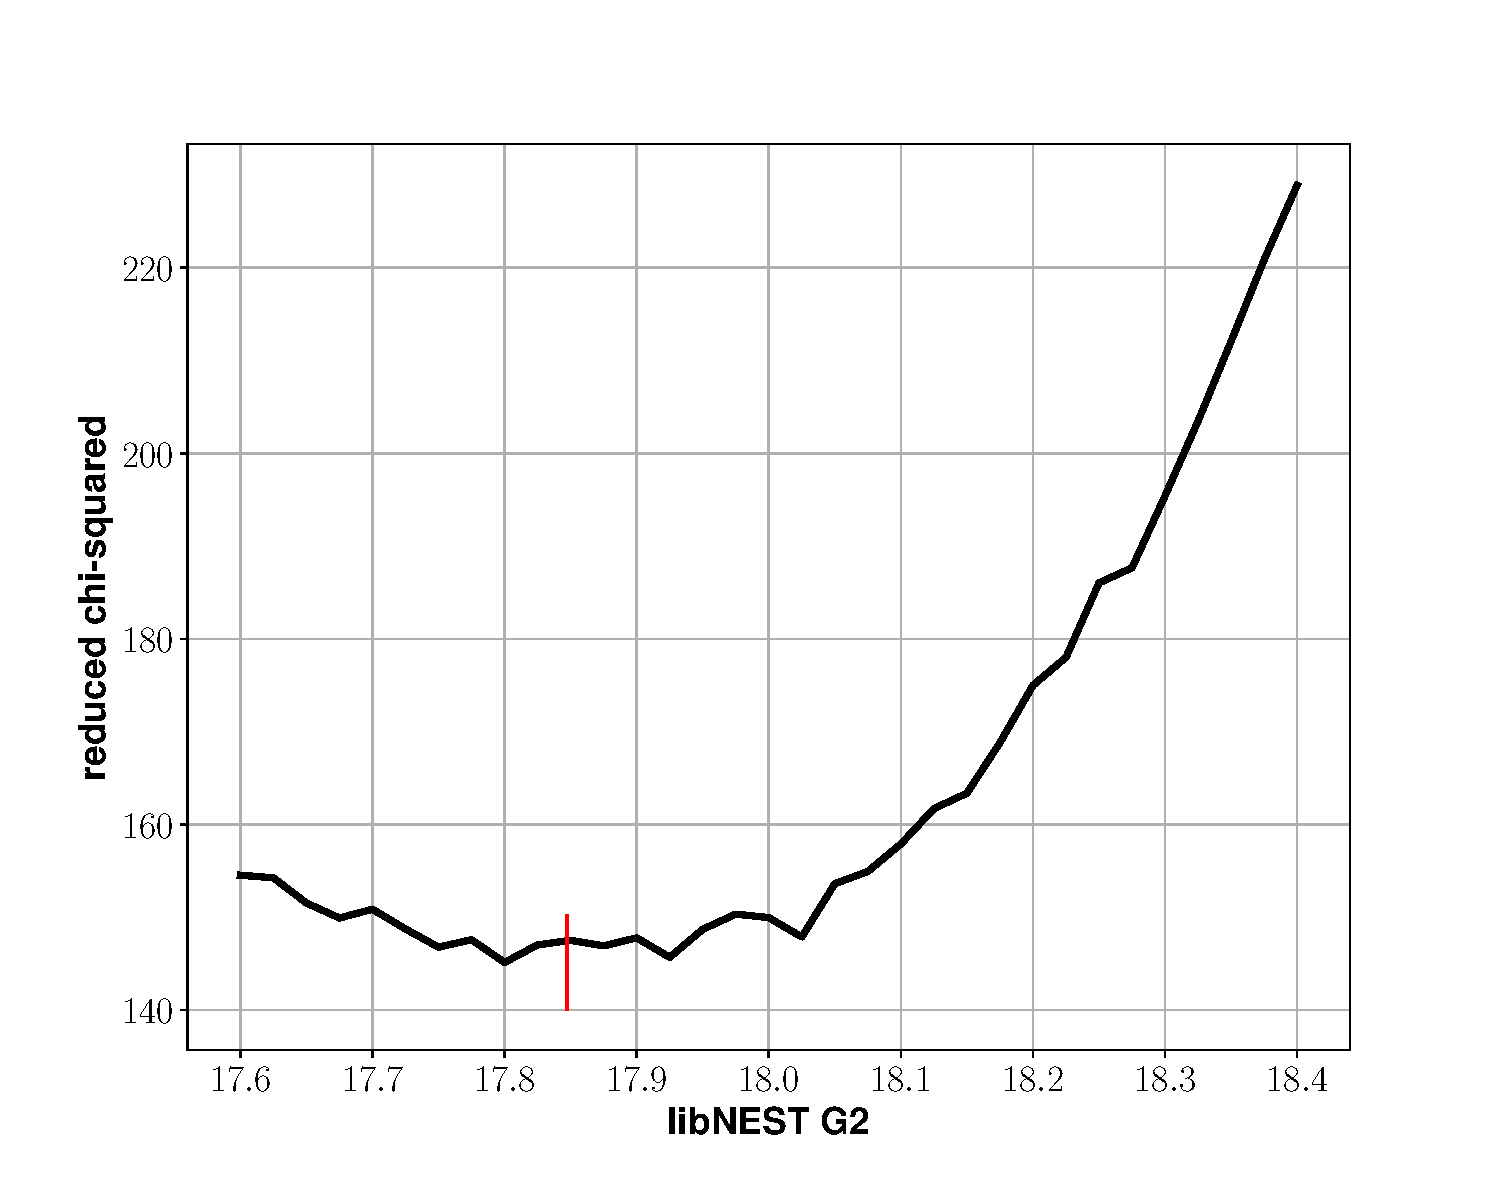
\includegraphics[width=\textwidth]{Figures/S2tail_g2fit_z.pdf}
  %\label{}
\end{subfigure}%
\begin{subfigure}{0.5\textwidth}
  \centering
  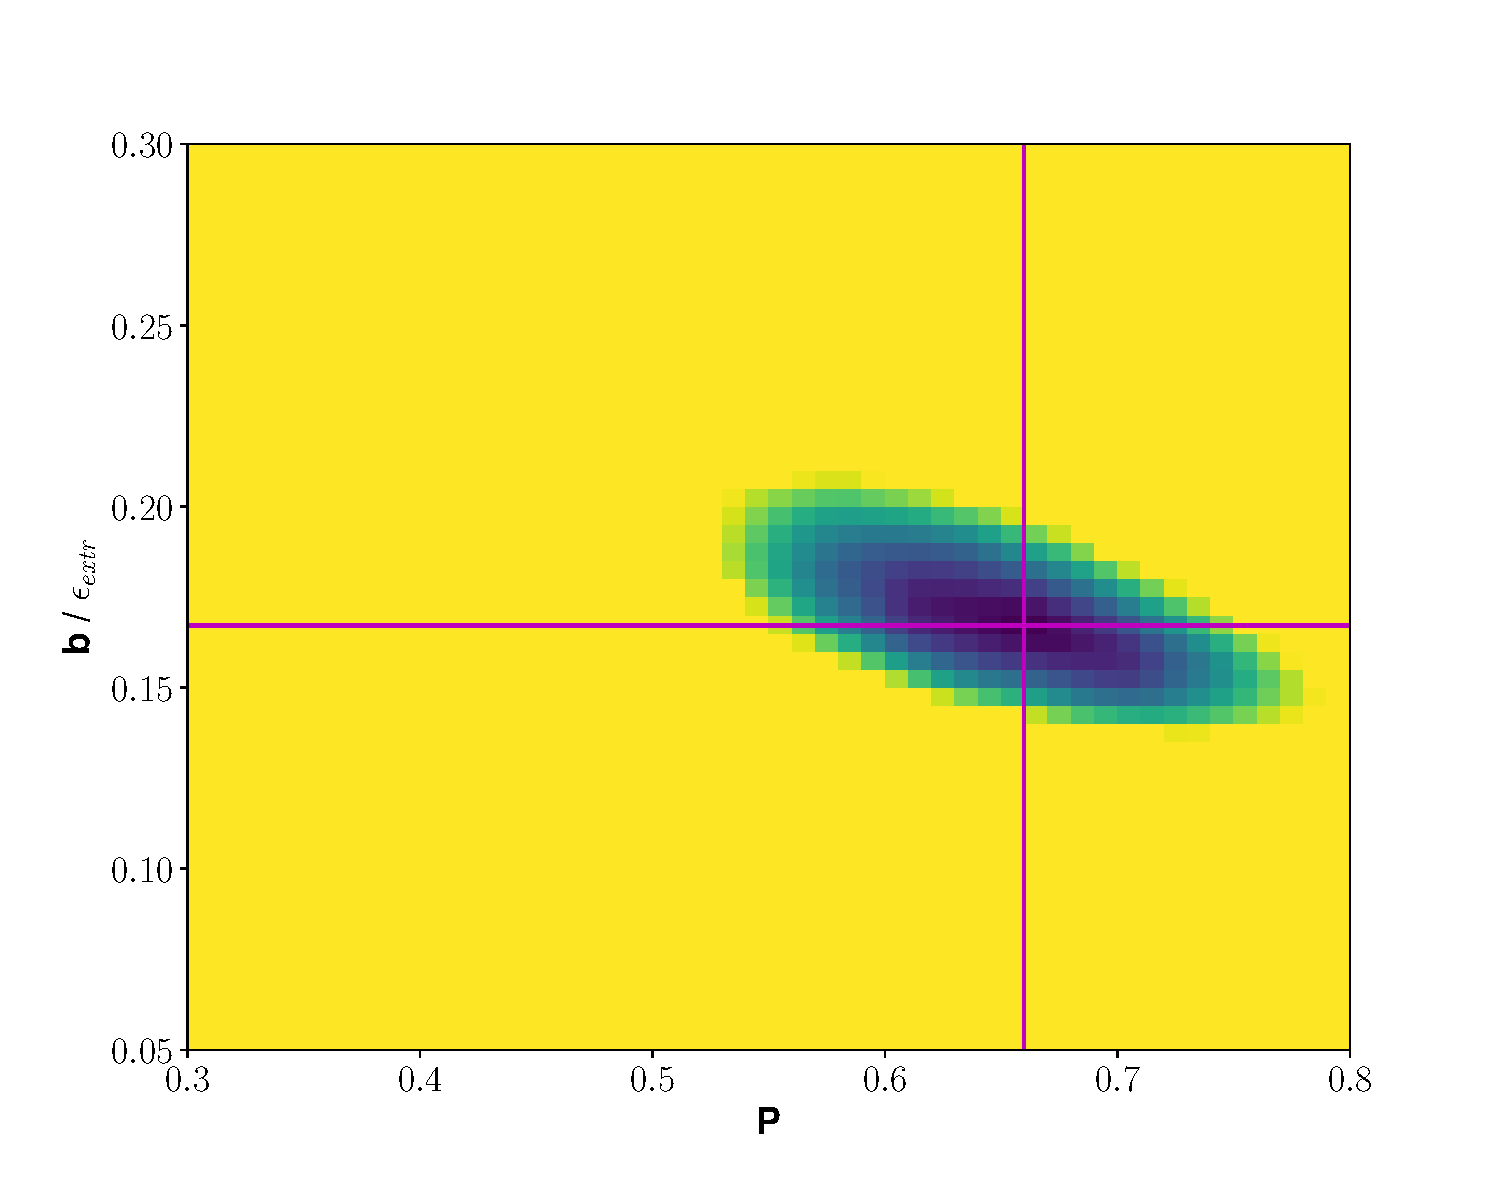
\includegraphics[width=\textwidth]{Figures/S2tail_heatmap_z.pdf}
  %\label{fig:intlin}
\end{subfigure}
\begin{subfigure}{0.5\textwidth}
  \centering
  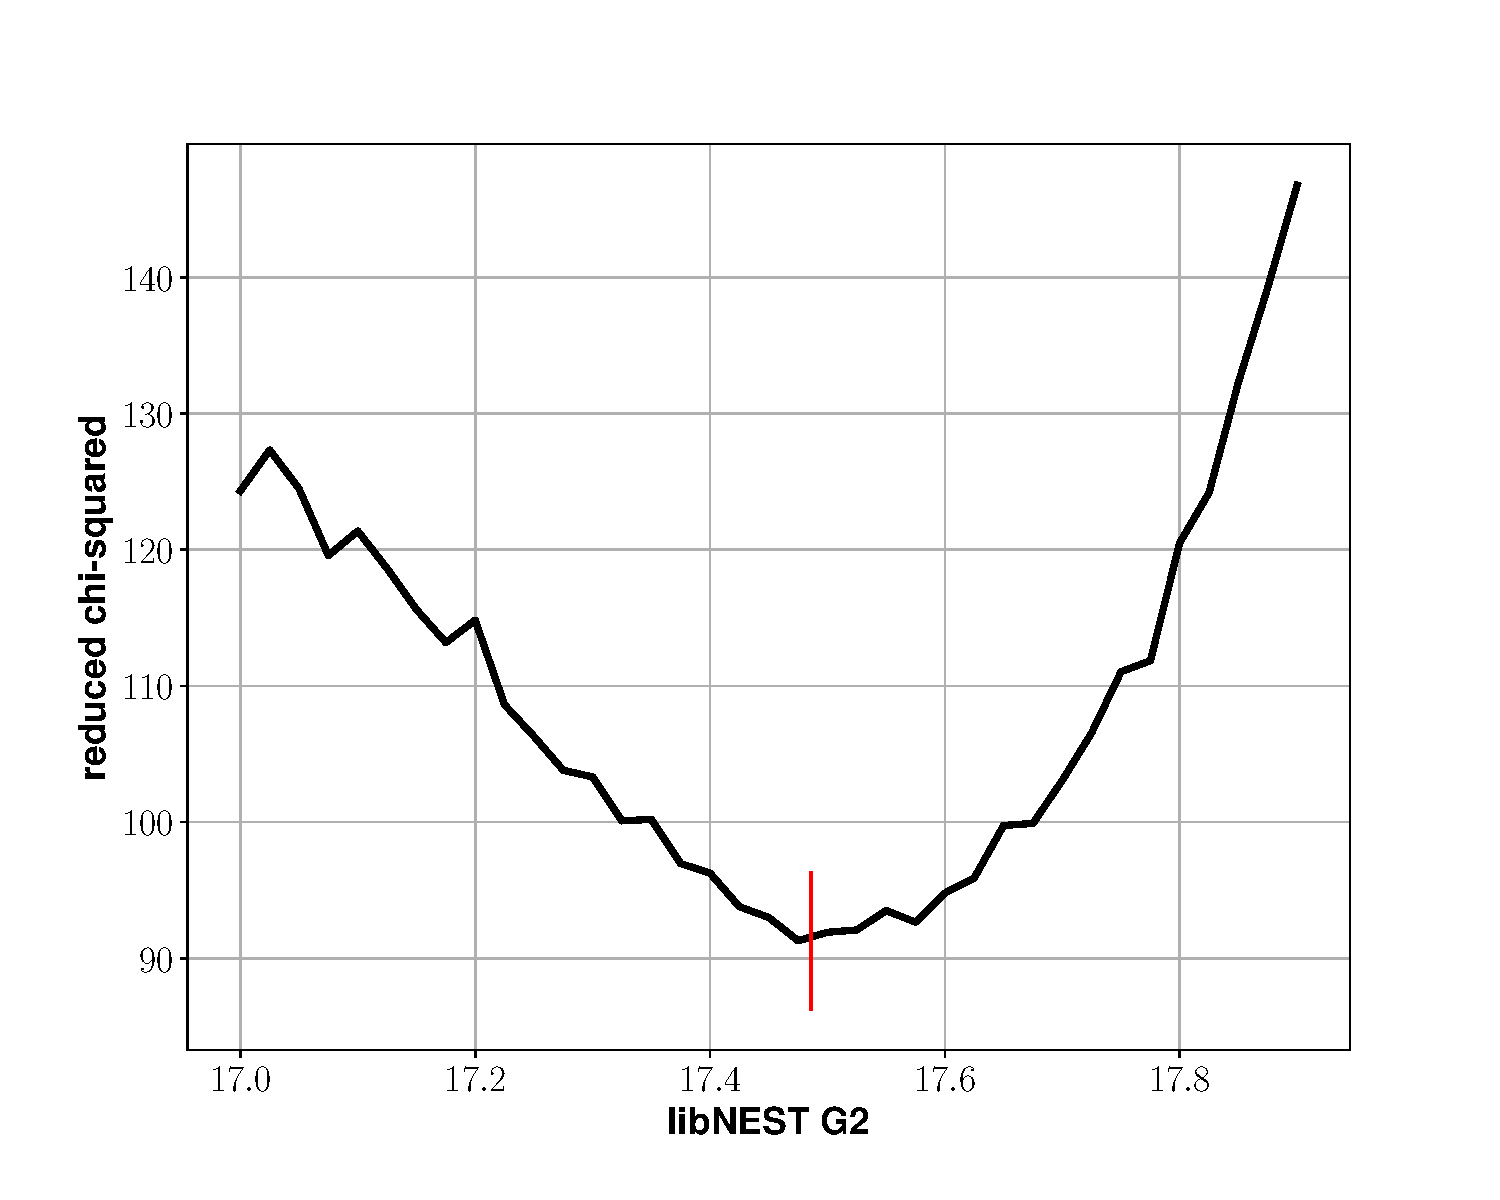
\includegraphics[width=\textwidth]{Figures/S2tail_g2fit_dcm.pdf}
  %\label{}
\end{subfigure}%
\begin{subfigure}{0.5\textwidth}
  \centering
  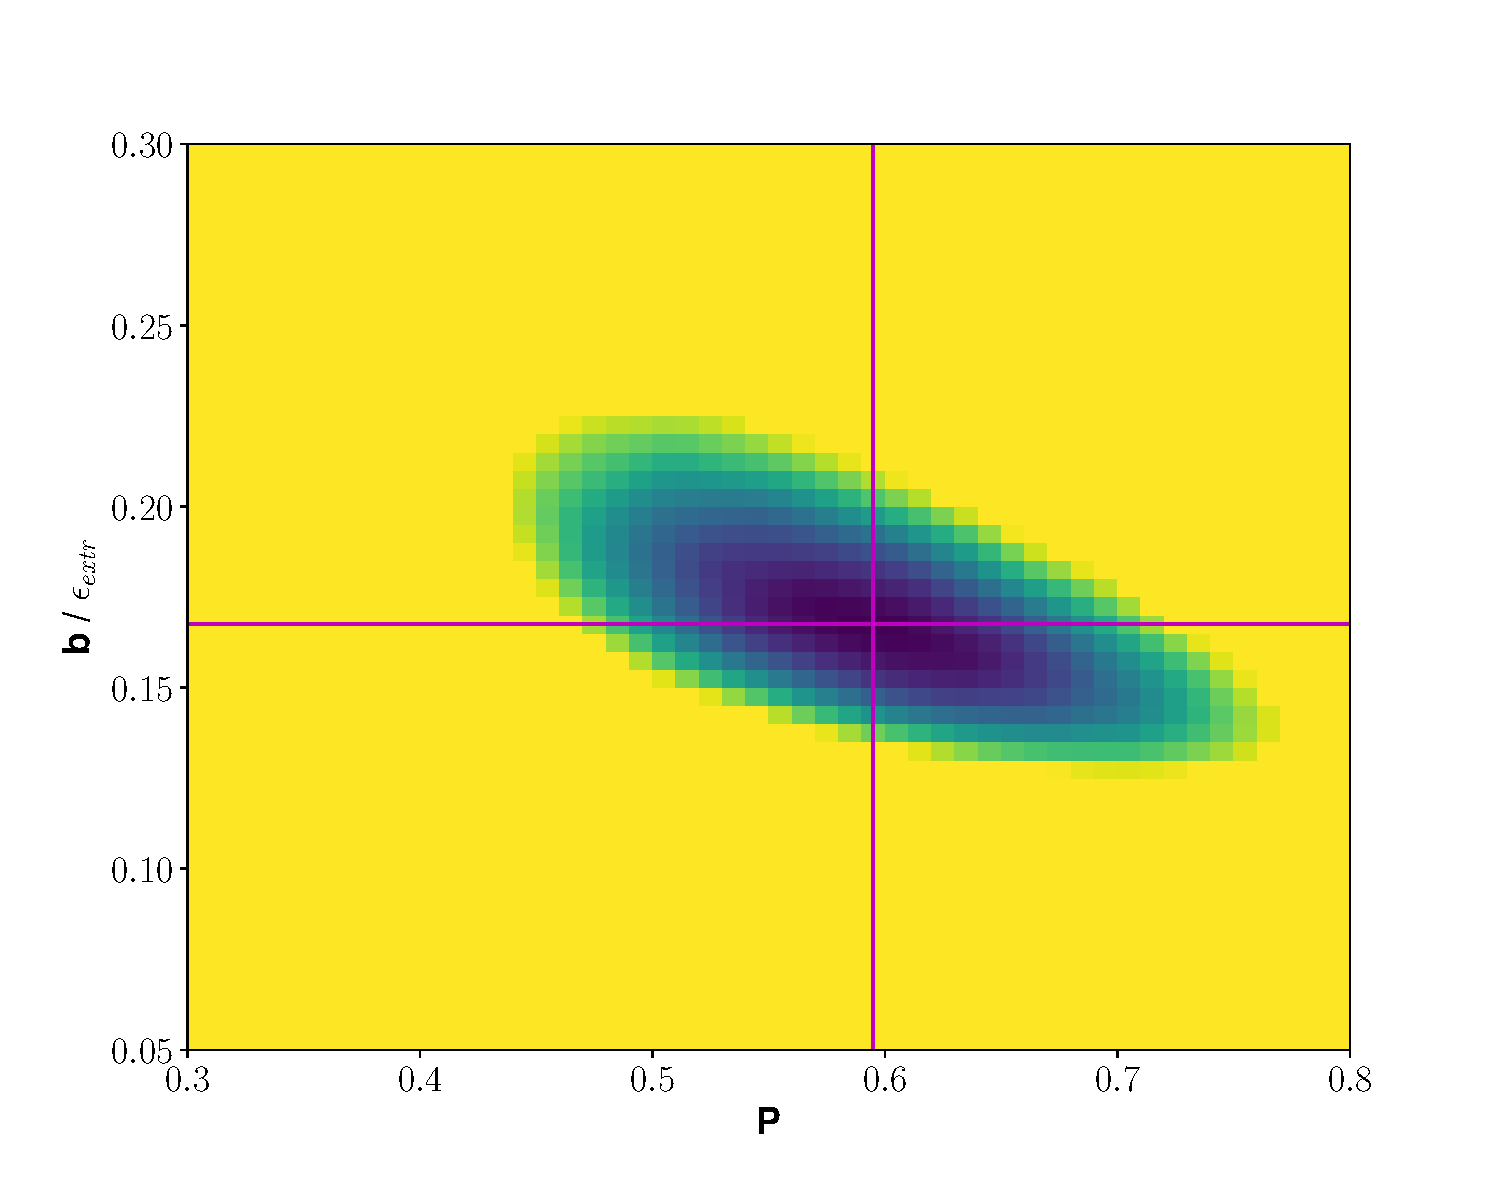
\includegraphics[width=\textwidth]{Figures/S2tail_heatmap_dcm.pdf}
  %\label{fig:intlin}
\end{subfigure}
\begin{subfigure}{0.5\textwidth}
  \centering
  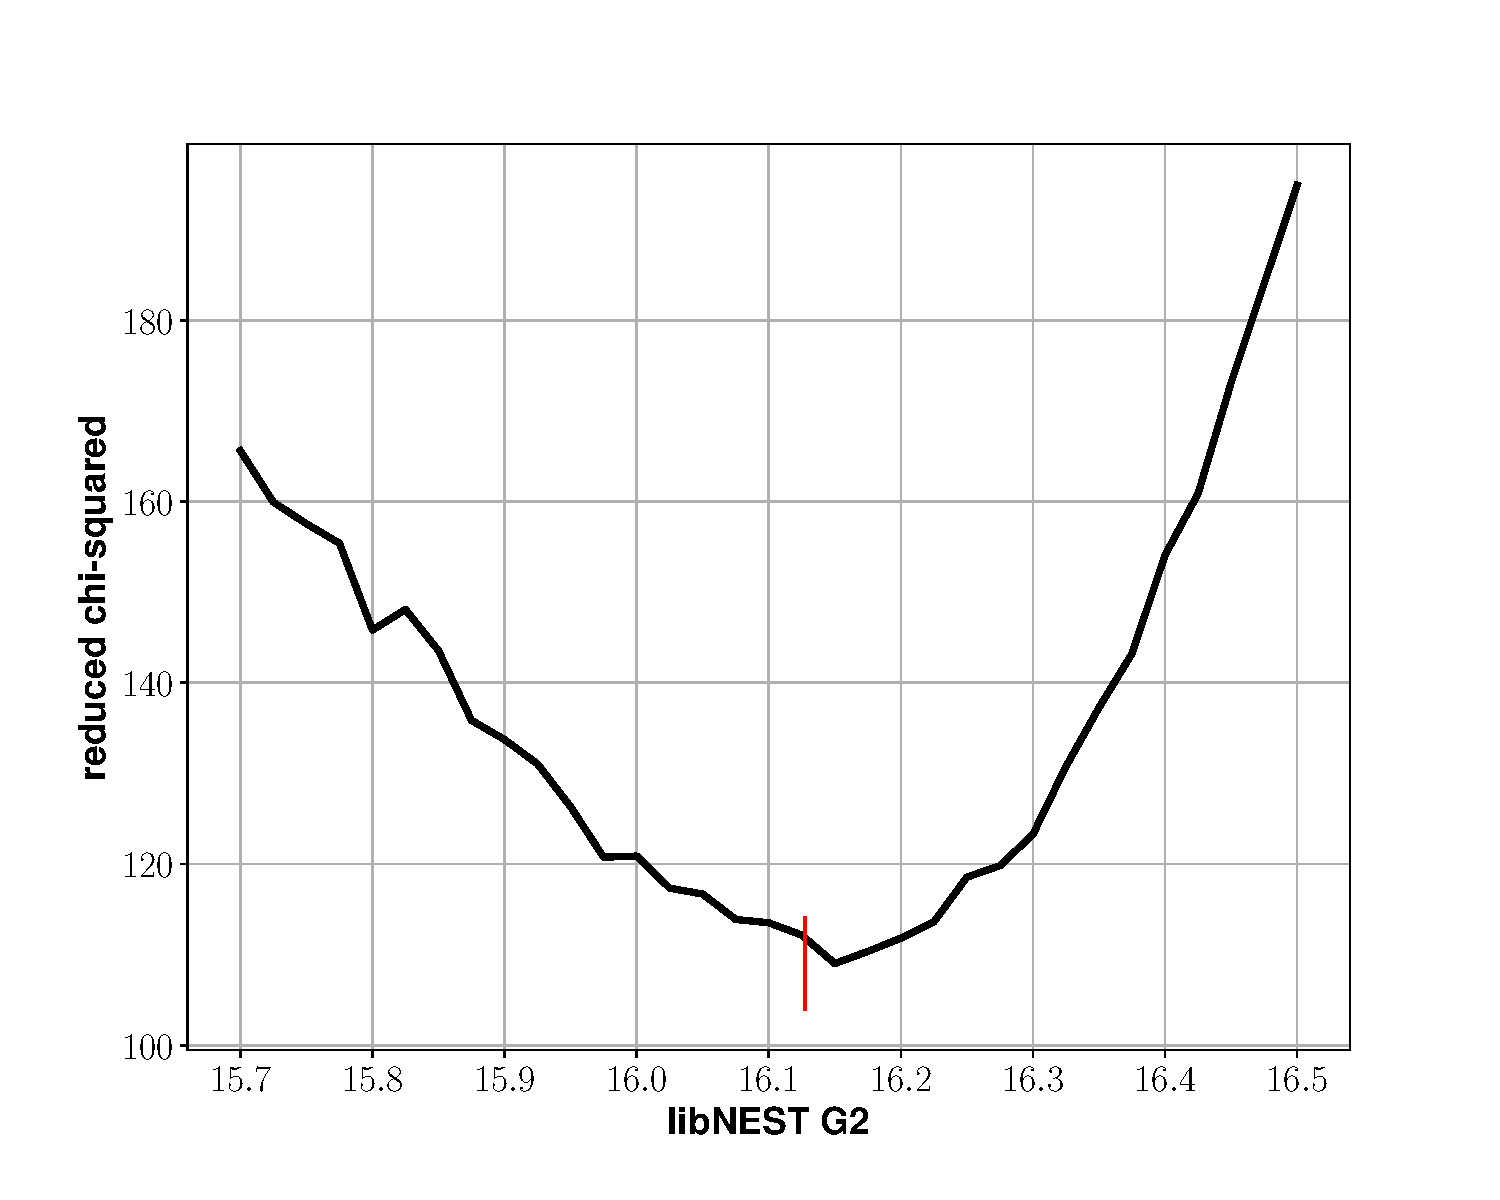
\includegraphics[width=\textwidth]{Figures/S2tail_g2fit_gfdcm.pdf}
  %\label{}
\end{subfigure}%
\begin{subfigure}{0.5\textwidth}
  \centering
  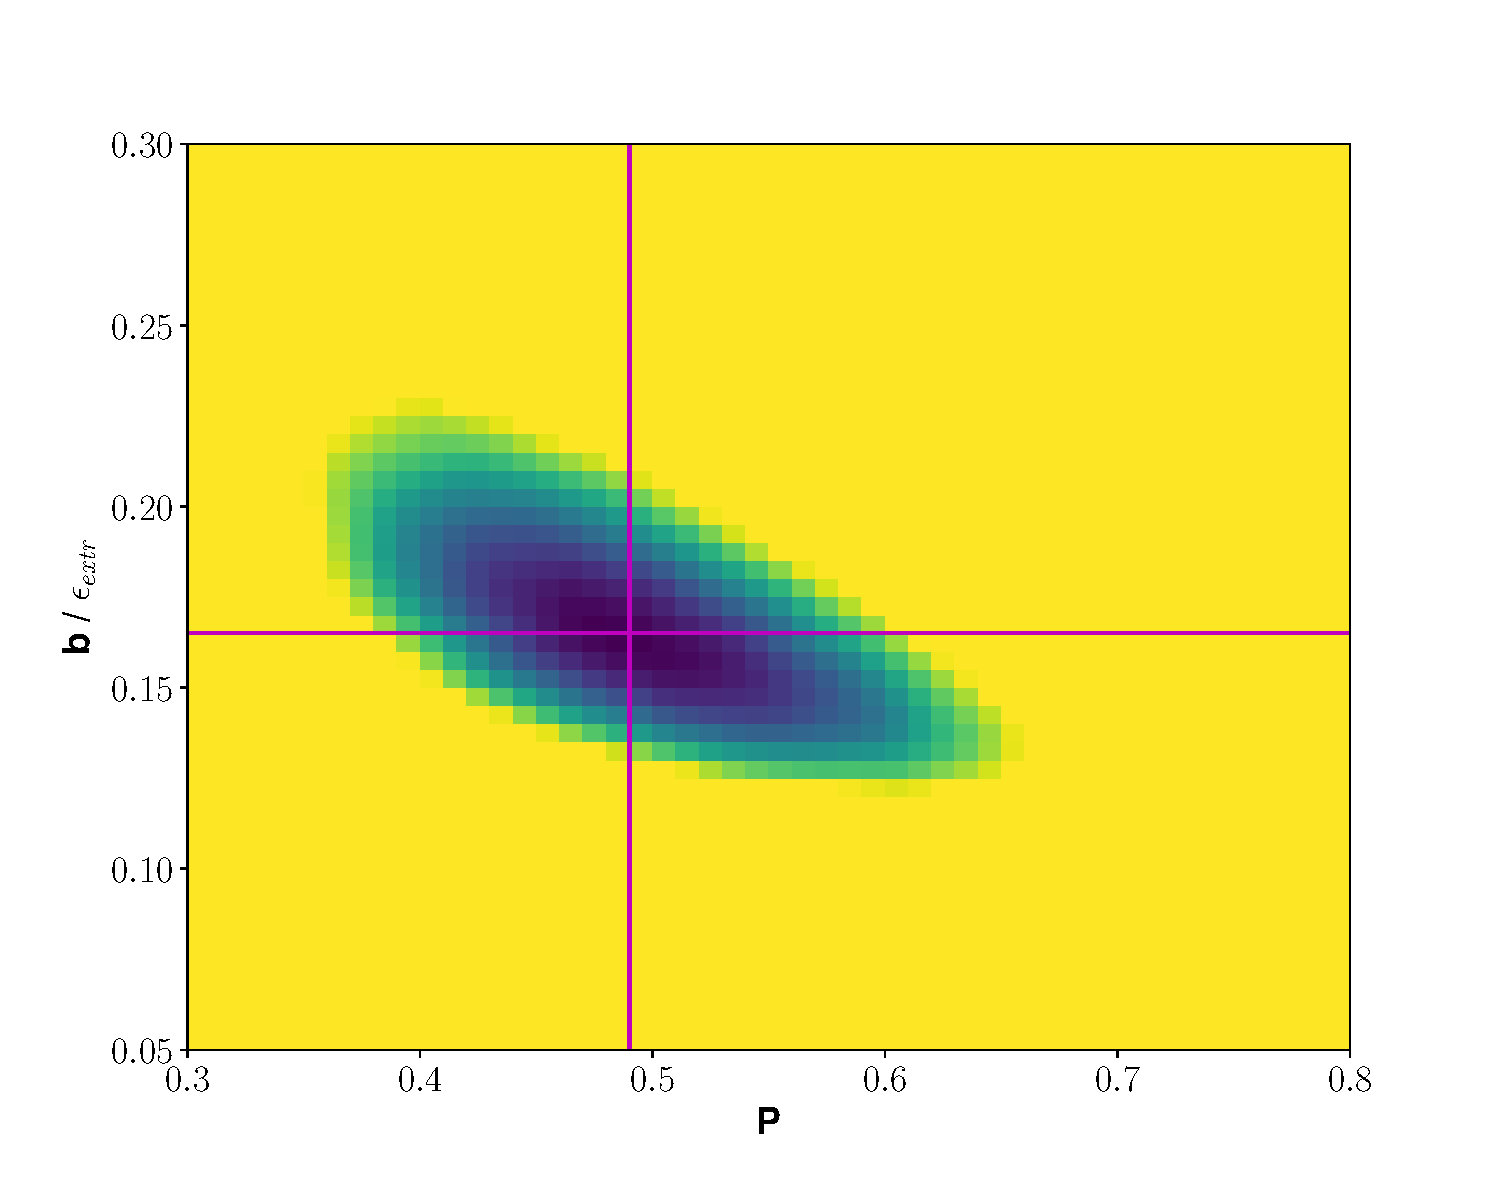
\includegraphics[width=\textwidth]{Figures/S2tail_heatmap_gfdcm.pdf}
  %\label{fig:intlin}
\end{subfigure}
\caption{Best fit results for the tail model for ``z'' (top), ``dcm'' (middle), and ``gfdcm'' (bottom) corrected data. The red an magenta lines indicate the best fit values calculated using the Metropolis algorithm.}
\label{fig:s2bestfit}
\end{figure}

We have a few observations in hand that help to motivate the development of a model of the S2 tails. First, it appears that not all events possess additional tail area, so we will try a model that assigns some probability, $P_{tail}$, that an event will be given additional area. We see from figure \ref{fig:E_spec_tails} that the size of the tails approximately follows an exponential distribution, and that the amplitude of the distribution is roughly proportional to the S2 size. With these observations we develop the model of S2 tails as follows:
\begin{enumerate}
\item Generate a random test variable, $T$, uniformly distributed between 0 and 1.
\item If $T>P_{tail}$, we set $N'_{e,extr}$=$N_{e,extr}$
\item If $T\leq P_{tail}$, we draw another random number $n_{tail}$ from an exponential distribution whose mean is equal to $b_{tail}$. We then set $N'_{e,extr}$=$N_{e,extr}(1+n_{tail})$.
\end{enumerate}
\begin{figure}[h!]
  \centering
  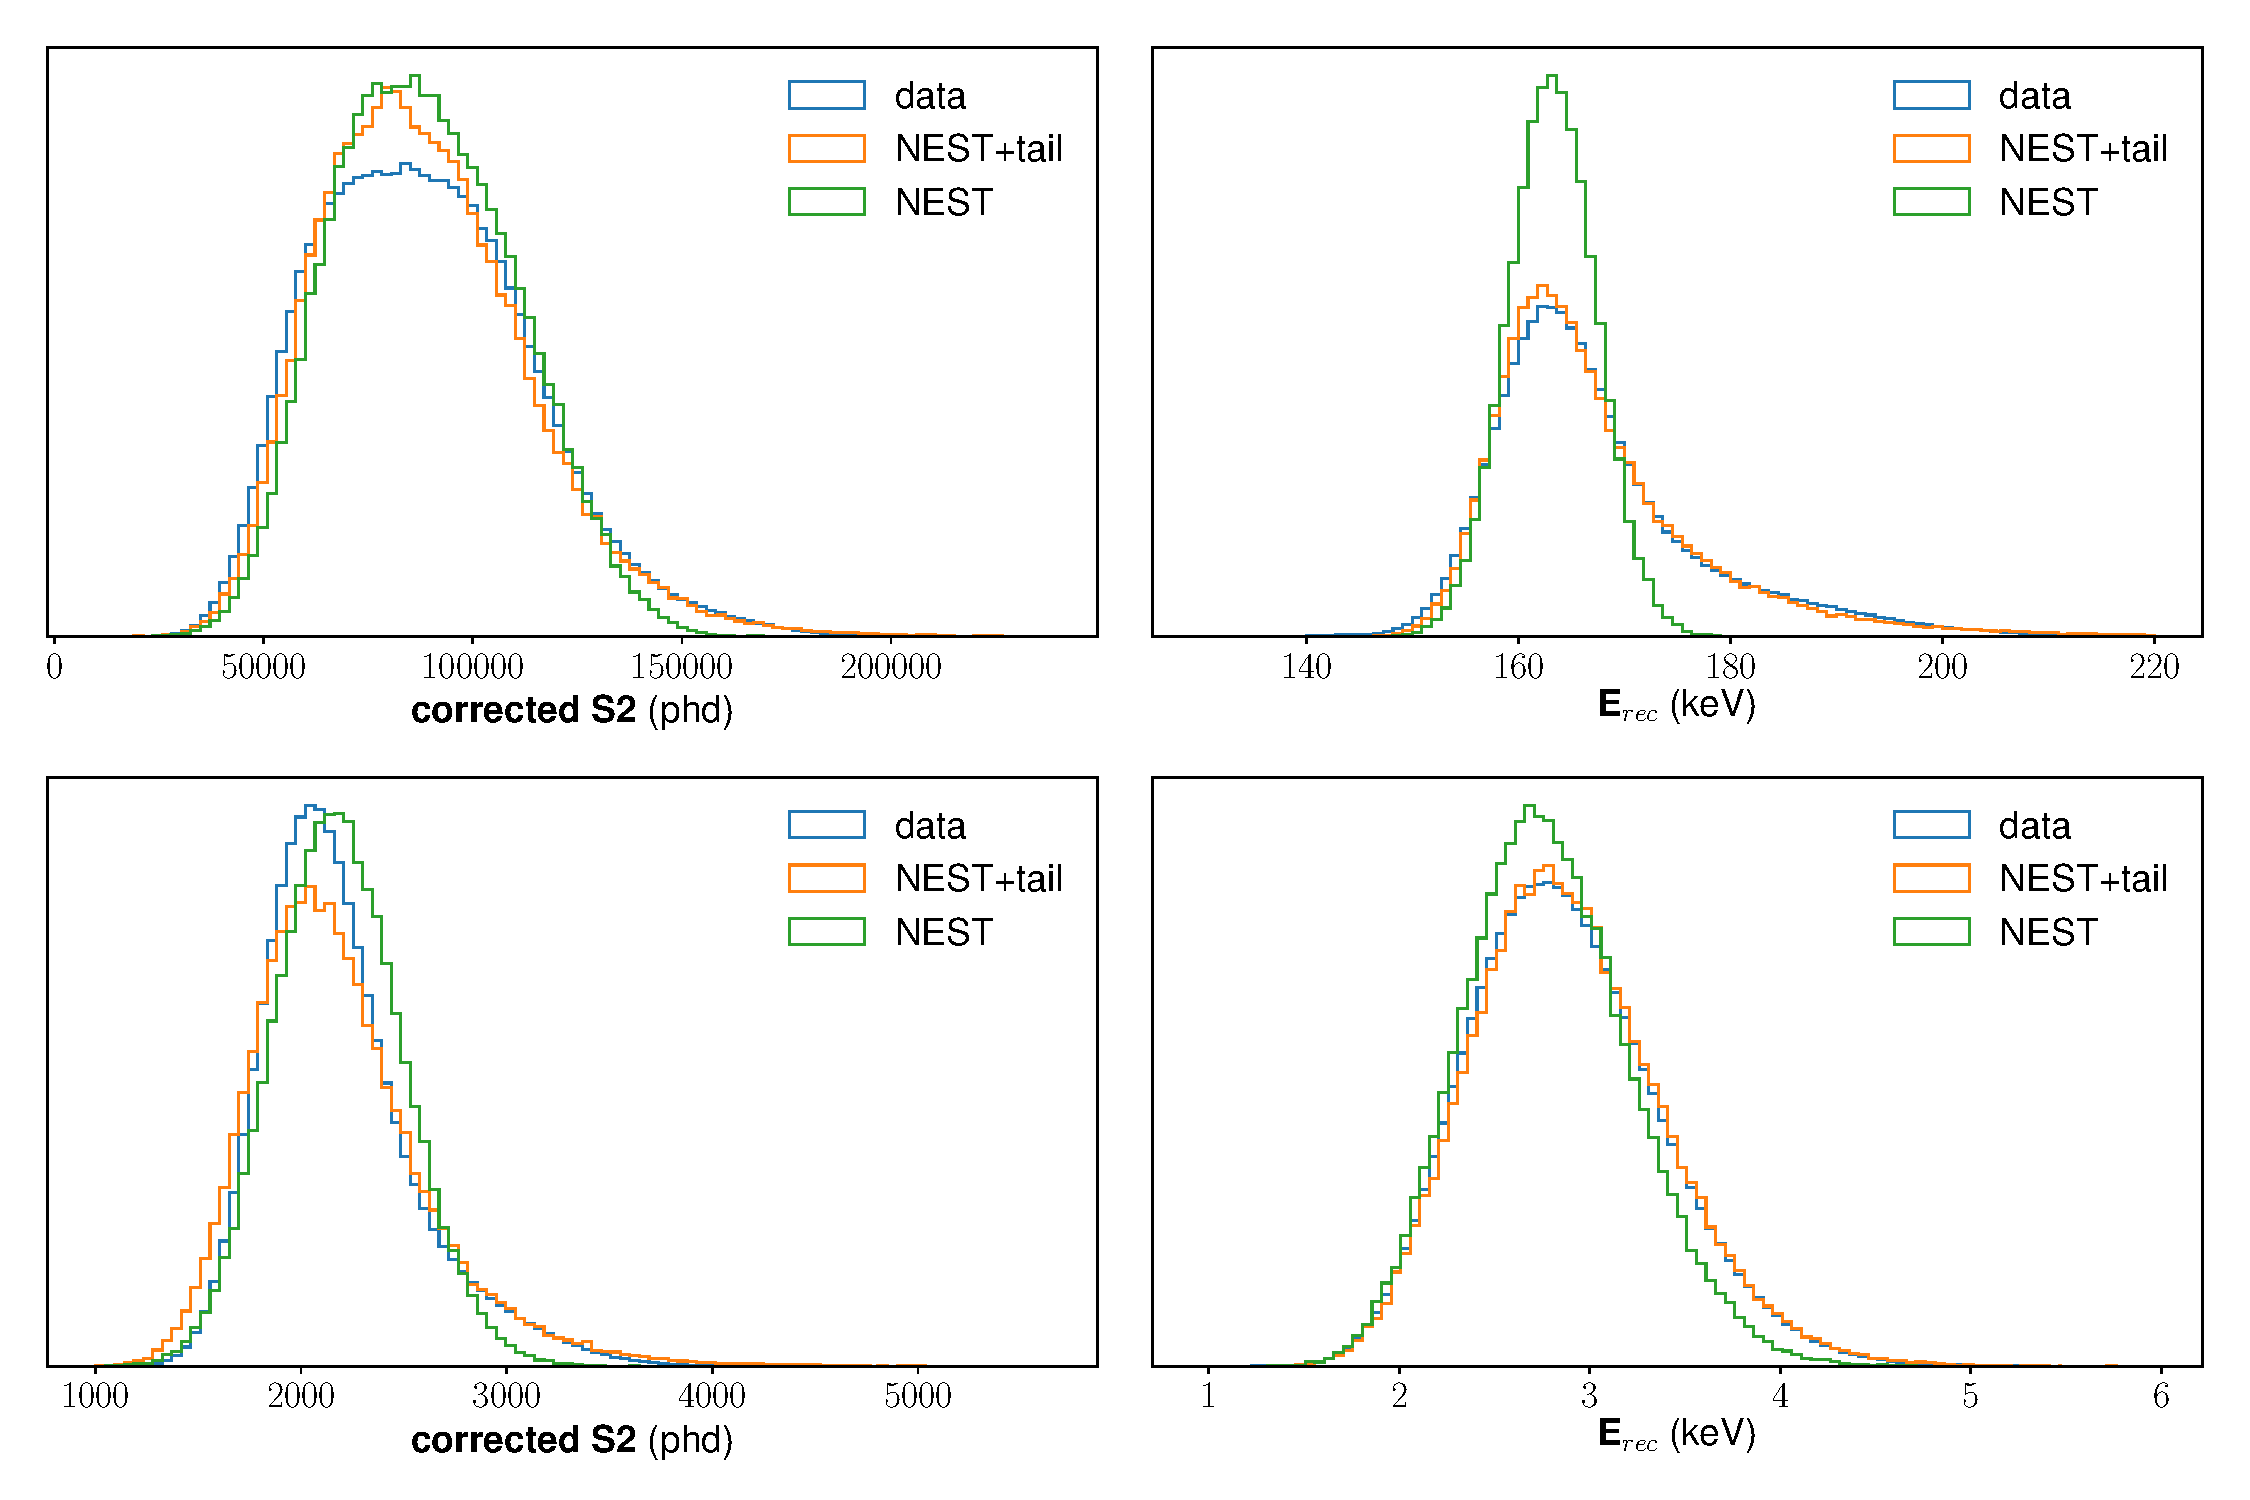
\includegraphics[width=\textwidth]{Figures/S2tail_hists_z.pdf}
  %\label{fig:intlin}
\caption{Best-fit spectra for ``z'' corrected data. The top plots are for the xenon-131m data, and the lower plots are for the argon-37 data. The green histogram, labeled ``NEST'', is the libNEST simulation with no S2 tail model added. The orange histogram. labeled ``NEST+tail'' is the libNEST model, plus the model of the S2 tails described in this section. The blue histogram shows what is observed in data. The spectra are calculated for 50 to 300 microseconds drift time.  }
\label{fig:s2bestfit_spec_z}
\end{figure}

This model is then dependent on three parameters, $P_{tail}$, $b_{tail}$, and the ``true'' value of G2, which needs to be input into the libNEST model. The G2 values as measured in figure \ref{fig:dt_doke_plot} will artificially high because of the pathological S2 area added by the tails. By varying these three parameters, we can optimize the model until it reproduces the observed energy spectra. 
\begin{figure}[h!]
  \centering
  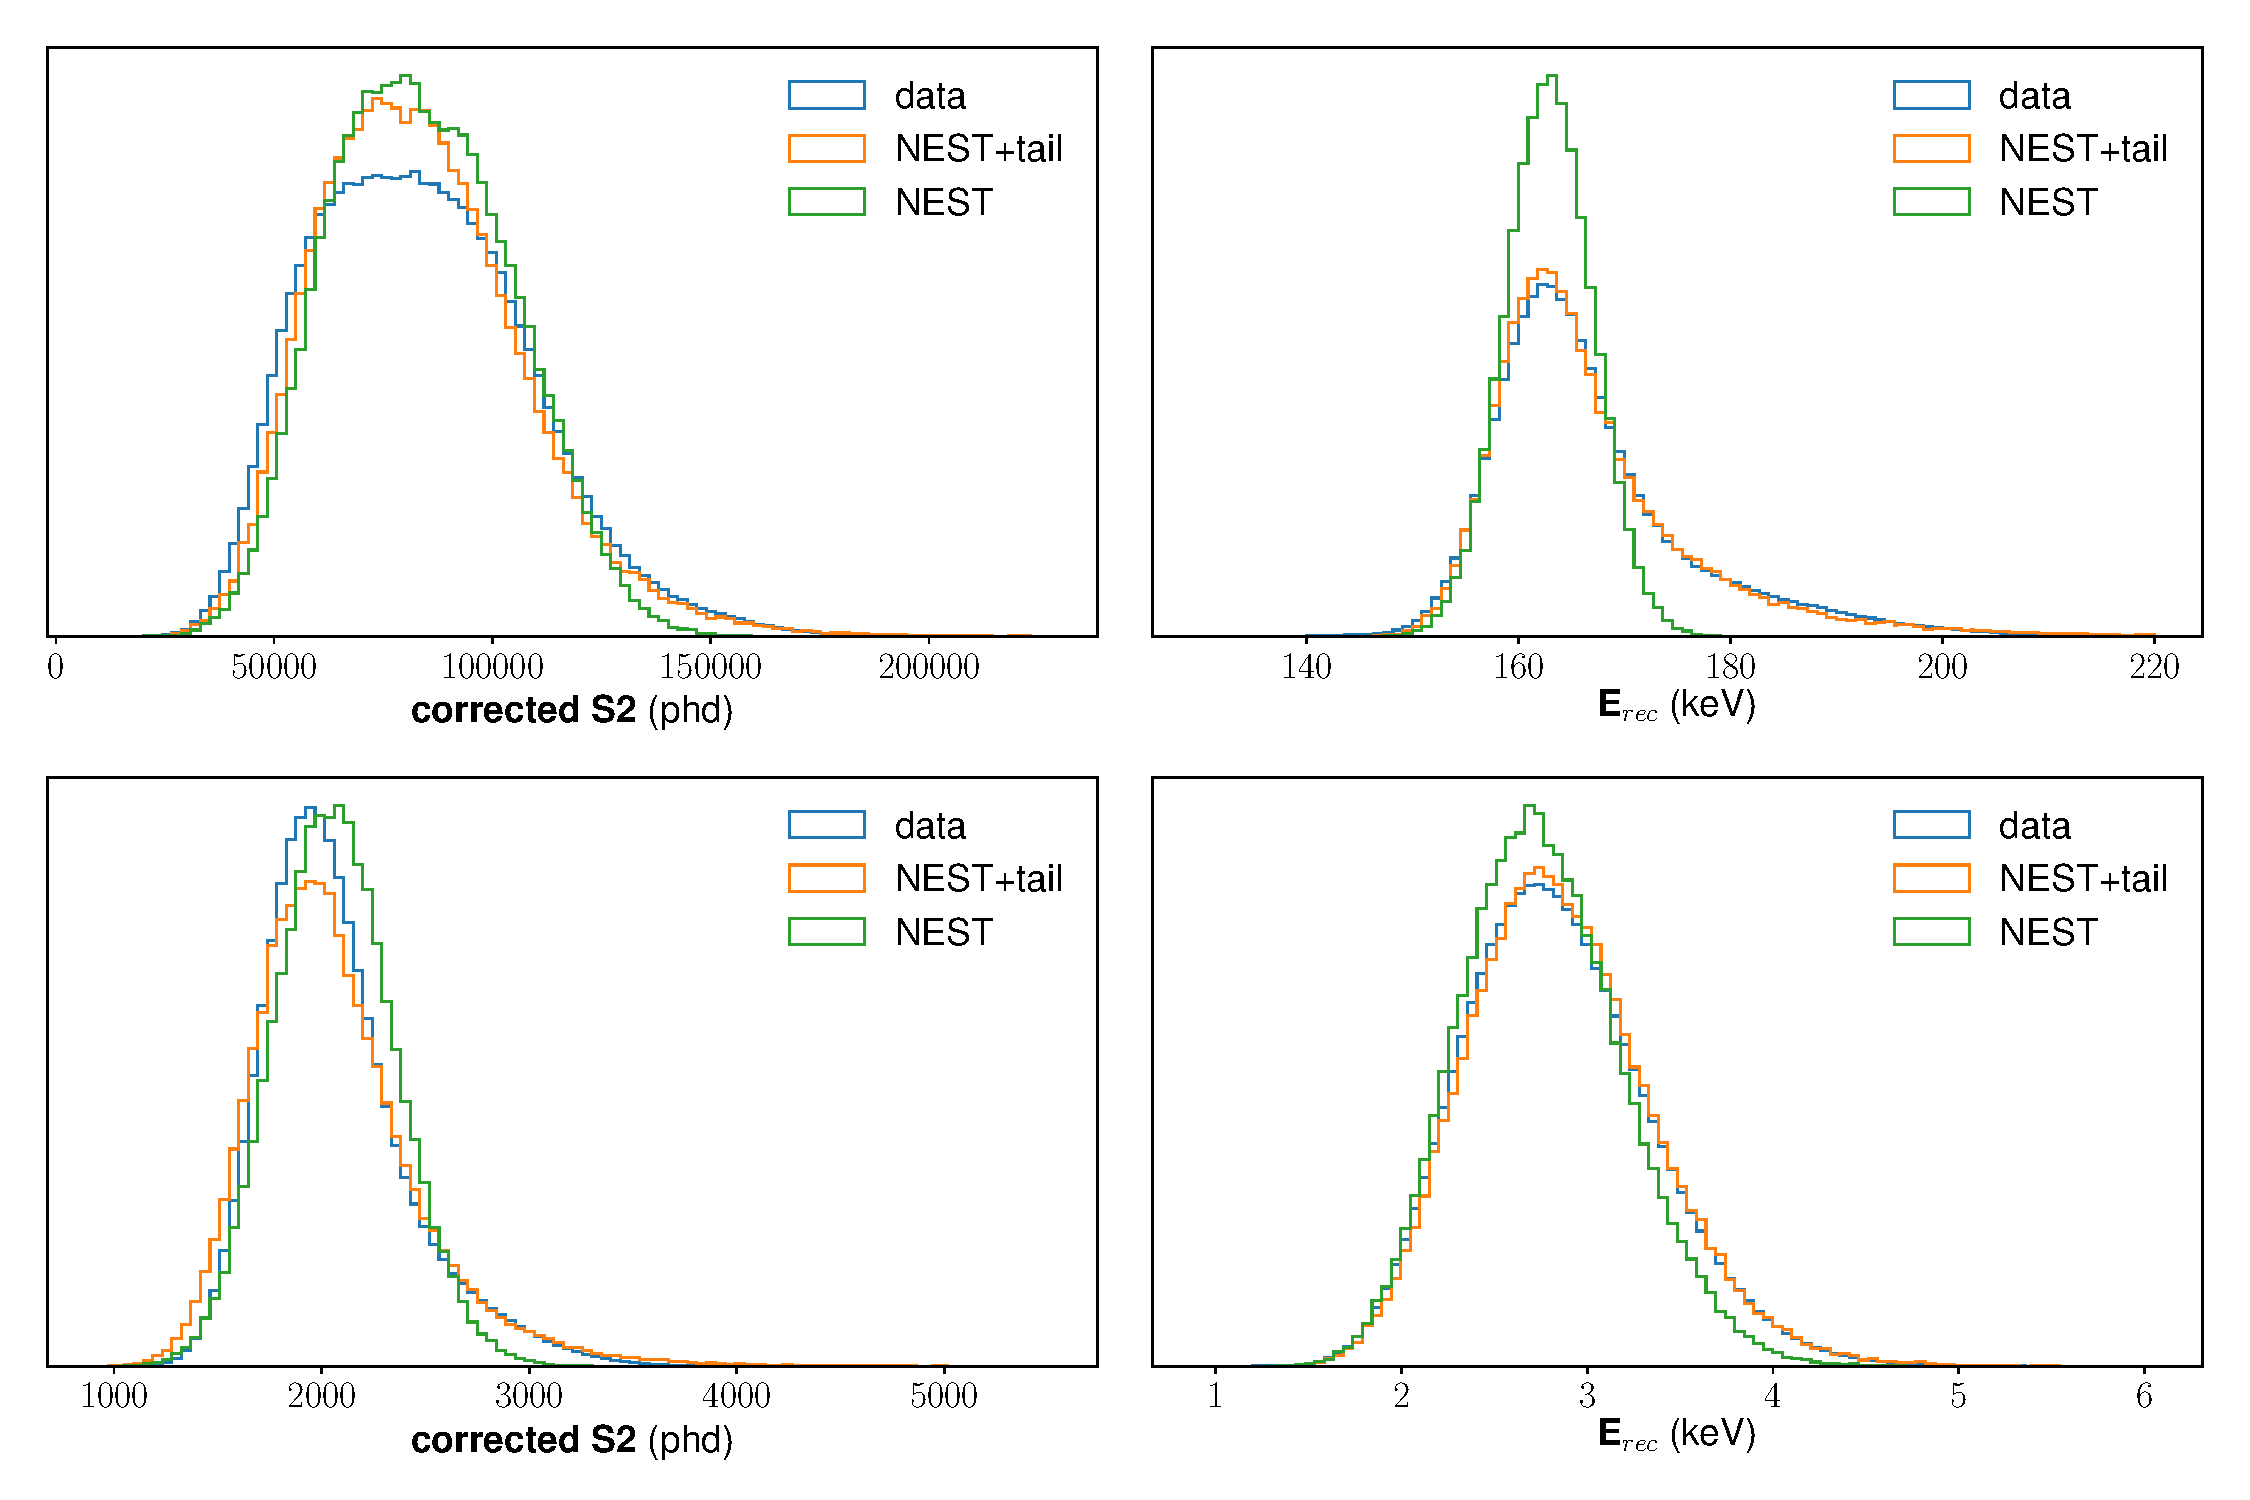
\includegraphics[width=\textwidth]{Figures/S2tail_hists_dcm.pdf}
  %\label{fig:intlin}
\caption{Best-fit spectra for ``dcm'' corrected data.  The top plots are for the xenon-131m data, and the lower plots are for the argon-37 data. The green histogram, labeled ``NEST'', is the libNEST simulation with no S2 tail model added. The orange histogram. labeled ``NEST+tail'' is the libNEST model, plus the model of the S2 tails described in this section. The blue histogram shows what is observed in data. The spectra are calculated for 50 to 300 microseconds drift time. }
\label{fig:s2bestfit_spec_dcm}
\end{figure}


We use our argon-37 and xenon-131m spectra as reference, calculating the $\chi^2$ difference between the libNEST S2 and reconstructed energy spectra, and those measured in data. We first scan across the parameters to locate the approximate location of the optimal parameters. This grid scan uses a modified model for computational convenience. Instead of adding the tail area to to $N_{e,extr}$, we add it to the final S2 area. Since this modified is applied after the extraction efficiency is modeled, the fractional tail area, $n_{S2,tail}$ will be drawn from an exponential distribution with a mean of $b_{tail}/\epsilon$.

\begin{figure}[h!]
  \centering
  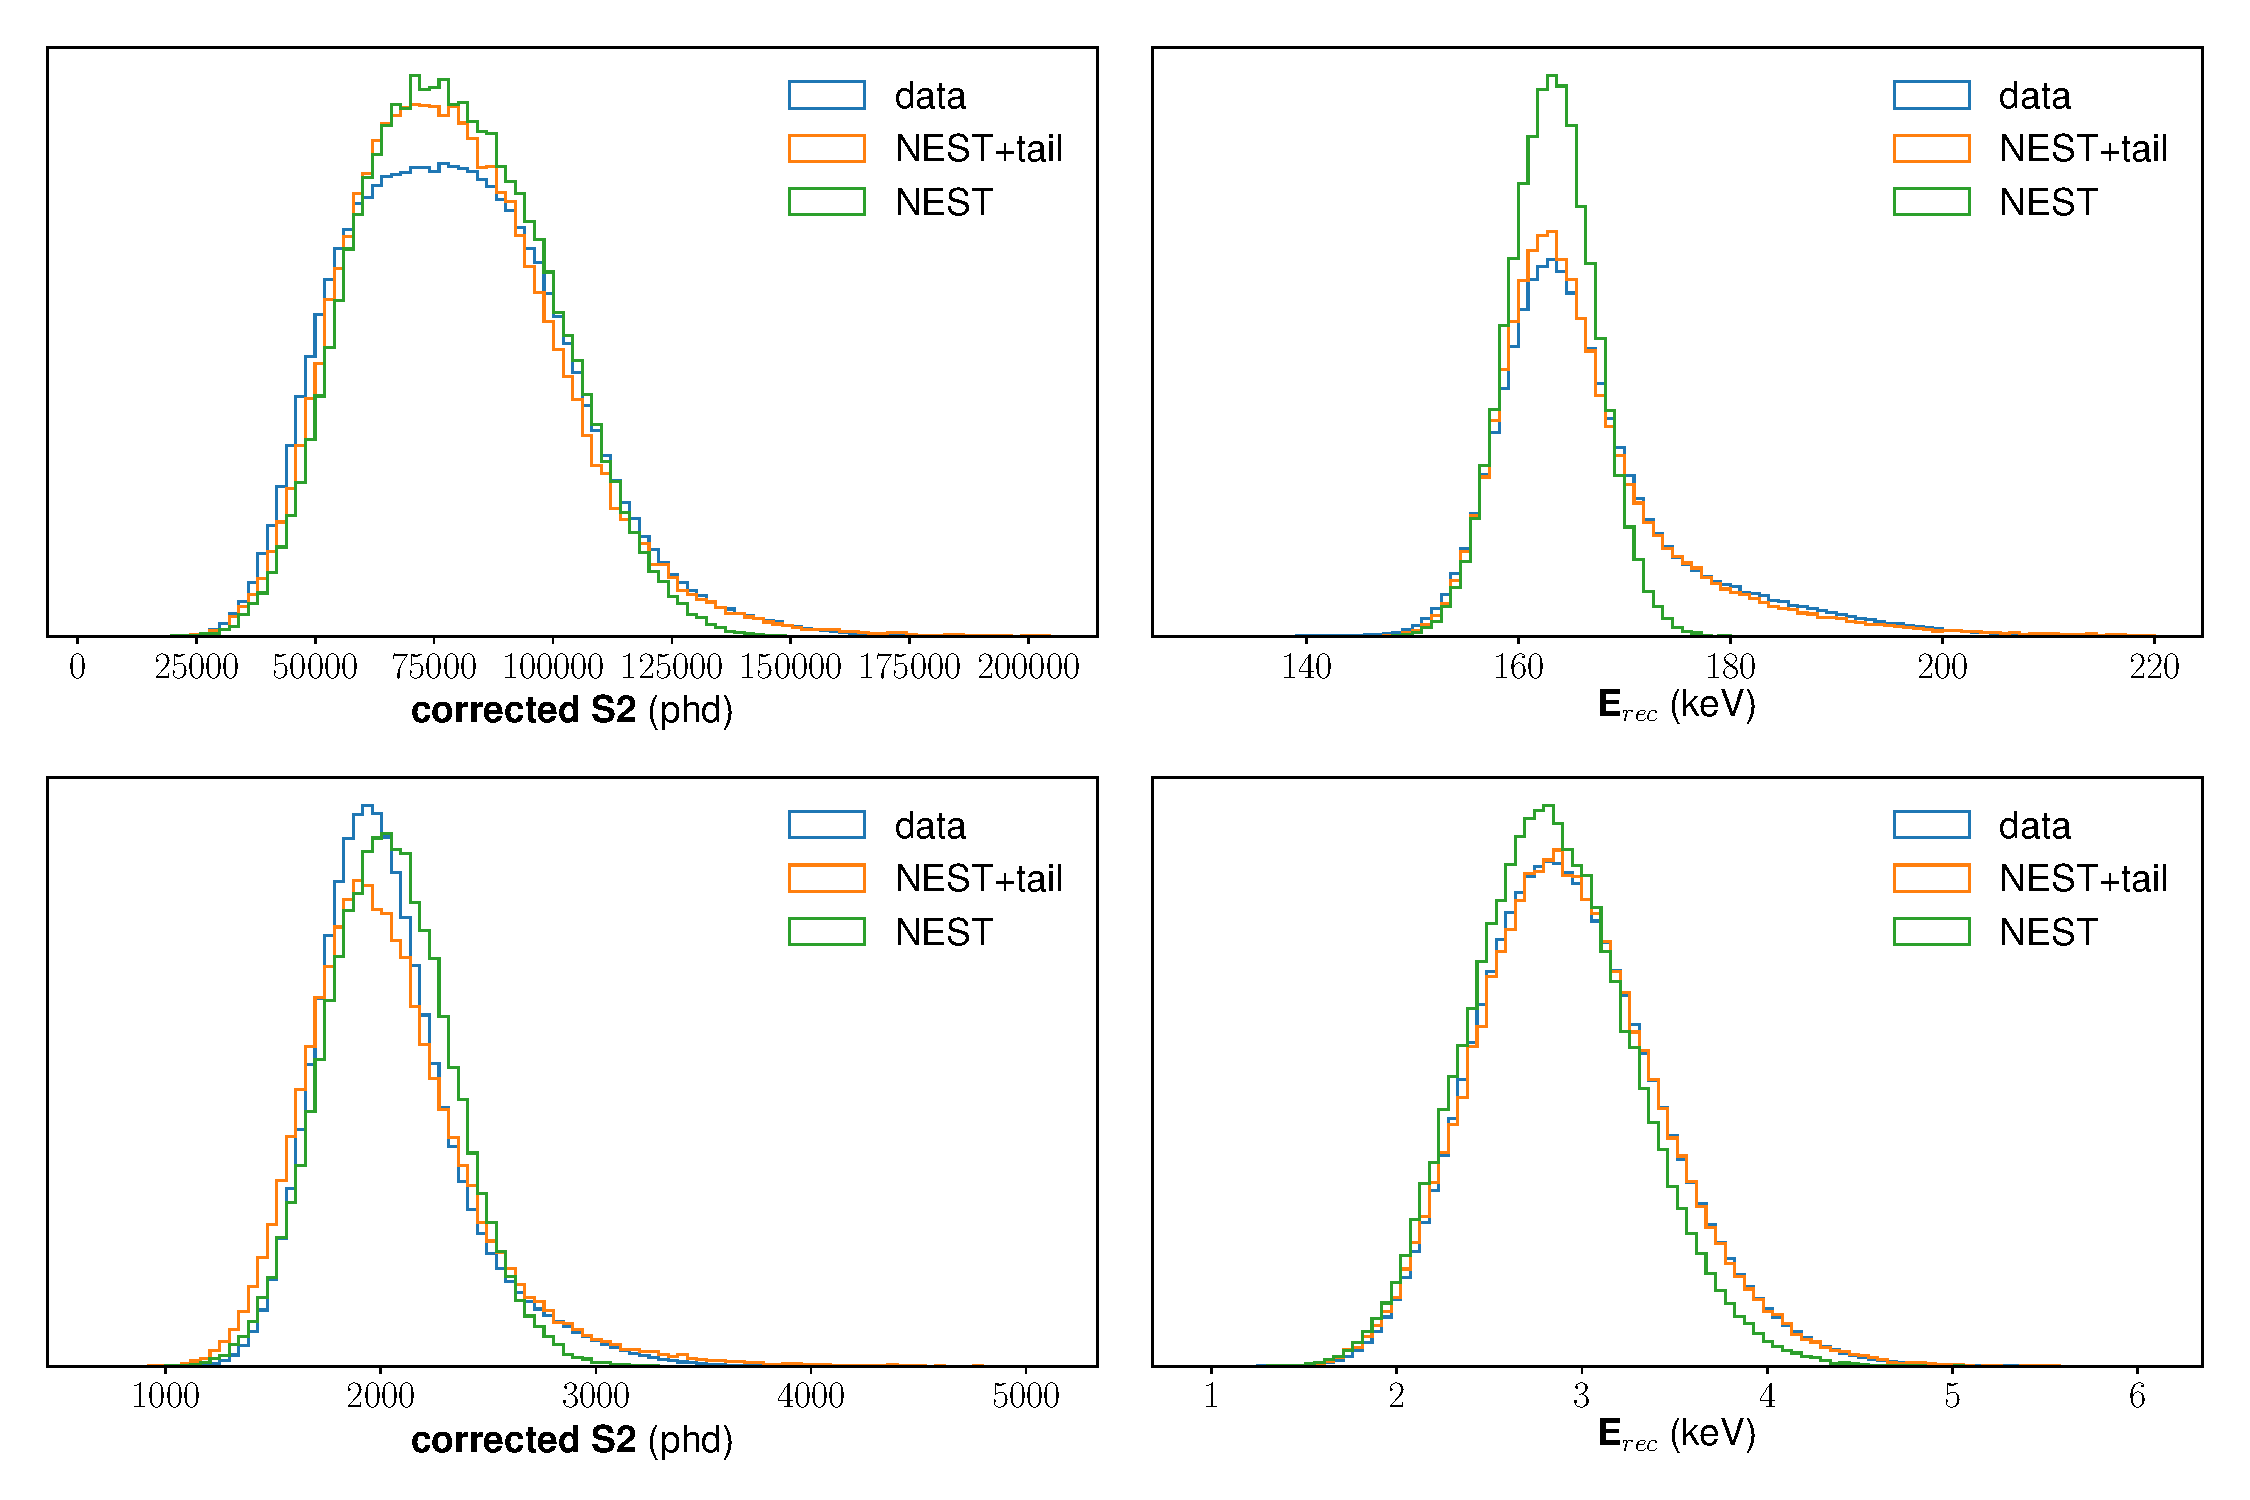
\includegraphics[width=\textwidth]{Figures/S2tail_hists_gfdcm.pdf}
  %\label{fig:intlin}
\caption{Best-fit spectra for ``gfdcm'' corrected data. The top plots are for the xenon-131m data, and the lower plots are for the argon-37 data. The green histogram, labeled ``NEST'', is the libNEST simulation with no S2 tail model added. The orange histogram. labeled ``NEST+tail'' is the libNEST model, plus the model of the S2 tails described in this section. The blue histogram shows what is observed in data. The spectra are calculated for 50 to 300 microseconds drift time. In order to account for an error in the yields, the peak location of the simulated S2 spectrum is adjusted to match that of the data spectrum.}
\label{fig:s2bestfit_spec_gfdcm}
\end{figure}

After the grid scan locates the approximate minimum, we then apply the Metropolis algorithm to fine tune the fit\cite{metropolis_1,metropolis_2}. For this algorithm, we use the model as we initially described it. For each iteration, we draw a new set test parameters from a normal distribution centered at the values of the previous iteration. These normal distributions have standard deviations of  0.005 for $b_{tail}$, 0.01 for $P_{tail}$, and 0.05 for $G2_{true}$. We then accept the new values of the parameters with a probability of $P_{accept}=\min(1,\exp(-(\chi_i^2-\chi_{i-1}^2)/2))$. We run at least 1000 iterations and allow for a burn-in period of 200 iterations. We take the best-fit values of the parameters to be equal mean of the iterations excluding the burn-in period.

\begin{table}[h!]
\centering
    \begin{tabular}{ c | c | c | c | c | c | c }
    \hline
    Correction & b$_{tail}$ & $\pm$ & P$_{tail}$ & $\pm$  & G2$_{true}$ & $\pm$ \\
    \hline \hline
    z & 0.112 & 0.003 & 0.73 & 0.02 & 17.6 & 0.05\\
    \hline
    dcm & 0.116 & 0.004 & 0.63 & 0.02 & 17.36 & 0.04 \\
    \hline
    gfdcm & 0.109 & 0.004 & 0.53 & 0.02 & 16.02 & 0.03 \\
    \hline
    \end{tabular}
    \caption{Best fit results for the S2 tail model.}
    \label{tab:s2bestfit}
\end{table}

We apply this fitting method to the three corrections methods we are testing; ``z'', ``dcm'', and ``gfdcm''. The results of the fit are shown in figure \ref{fig:s2bestfit}, as well as in table \ref{tab:s2bestfit}. The data and NEST+tail energy histograms are in good agreement, indicating that our tail model is successful. There is some disagreement in the S2 spectra near the peak value. This is likely explained by incorrect values for the input recombination fluctuations. We will aim to better measure this input value in the next chapter.









